\newif\ifdevelop
%%%%%%%%%%%%%%%%%%%%%%%%%%%%%%%%%%%%%%%%%%%%%
%                                          %%
% Developmode ein bzw. ausstellen          %%
  \developtrue
% \developfalse
%%%%%%%%%%%%%%%%%%%%%%%%%%%%%%%%%%%%%%%%%%%%%
% Definition der Abgabeversion             %%
  \newcommand{\documentversion}{0.4.7}
%%%%%%%%%%%%%%%%%%%%%%%%%%%%%%%%%%%%%%%%%%%%%
\documentclass[ngerman]{scrreprt}
%
% - - - Allgemeine Parameter - - - -
%
% - - - Abgabedatum der Arbeit - - - 
\newcommand{\dateOfSubmission}{10. August 2018%
\importantTodo{Abgabedatum anpassen}
}
% - - - Autor - - - 
\newcommand{\authorOfWork}{Martin Leonard Haufs}
% - - - Matrikelnummer - - -
\newcommand{\matrikelnummer}{4015814}
% - - - Studiengang
\newcommand{\studiengang}{Scientific Programming}
% - - - Dokumententyp - - -
\newcommand{\documentTypeName}{Bachelorarbeit}
% - - - Titel der Arbeit
\newcommand{\documentTitle}{Multimediale Unterst\"utzung in der Medizinprodukteaufbereitung mittels Smartglasses}
% - - - Erstprüfer - - -
\newcommand{\erstpruefer}{Prof. Dr. Volker Sander}
% - - - Zweitprüfer - - - 
\newcommand{\zweitpruefer}{Dr. Mirco Vitr}
% - - - Dokumentenklasse - - - 
%
% - - - Header - - - 
%

% 1.5-facher Zeilenabstand:
\usepackage[onehalfspacing]{setspace} 

\usepackage[utf8]{inputenc}
\usepackage[ngerman]{babel}
% Durchgehende Nummerierung von Abbildungen über
% Chapter hinaus
%\usepackage{chngcntr}
%\counterwithout{figure}{chapter}
%
% Kommentare mit \comment{}-Umgebung
\usepackage{verbatim}
%
\usepackage[%
    backend=biber,
    style=numeric,
    %style=alphabetic,
    %citestyle=alphabetic-verb,
    %citestyle=numeric
    %sorting=ynt    % Sortierung nach Name des Autors
    sorting=none    % Sortierung nach Auftreten
]{biblatex}
%\addbibresource{data/bibliography.bib}
\addbibresource{Bachelorarbeit.bib}

\usepackage{fancyvrb}
\usepackage{listings}

\lstset{literate=%
  {Ö}{{\"O}}1
  {Ä}{{\"A}}1
  {Ü}{{\"U}}1
  {ß}{{\ss}}2
  {ü}{{\"u}}1
  {ä}{{\"a}}1
  {ö}{{\"o}}1
}


\usepackage{minted}
\usepackage[german]{fancyref}
\usepackage{enumitem}
\usepackage{array}
\usepackage{graphicx}
\usepackage{multicol}
%\usepackage{pgf-umlsd}
%\usepackage[pict2e]{struktex}
\usepackage{tikz}
%\usetikzlibrary{arrows,shadows}
%\usepackage{csvsimple}
%\usepackage{pgfplots}
\usepackage{filecontents}
%\usepackage{../daten/tikz-uml}

% Anführungsstriche mit \enquote{}-Umgebung
\usepackage[autostyle]{csquotes} 

% =============================
\usepackage[colorinlistoftodos,prependcaption,textsize=tiny]{todonotes}

% Hyperlinks in PDF-Version des Dokumentes. Option sagt, dass keine roten Boxen erzeugt werden sollen.
\usepackage[pdfborder={0 0 0}]{hyperref} 

% Todo commands
% https://mirror.hmc.edu/ctan/macros/latex/contrib/todonotes/todonotes.pdf
\newcommand{\insertMore}[1]{\todo[inline, color=green!40]{#1 ergänzen}}
\newcommand{\insertRef}[1]{\todo[color=blue!40]{#1 (Referenz fehlt)}}
\newcommand{\importantTodo}[1]{\todo[color=red!40]{#1 (Wichtig!)}}

% Programmcode


\begin{comment}

\usepackage{geometry}
\geometry{
  left=2.5cm,
  right=2.5cm,
  top=2cm,
  bottom=2cm,
  bindingoffset=5mm
}

\end{comment}

\definecolor{lightgray}{rgb}{0.95, 0.95, 0.95}
\definecolor{darkgray}{rgb}{0.4, 0.4, 0.4}
%\definecolor{purple}{rgb}{0.65, 0.12, 0.82}
\definecolor{editorGray}{rgb}{0.95, 0.95, 0.95}
\definecolor{editorOcher}{rgb}{1, 0.5, 0} % #FF7F00 -> rgb(239, 169, 0)
\definecolor{editorGreen}{rgb}{0, 0.5, 0} % #007C00 -> rgb(0, 124, 0)
\definecolor{orange}{rgb}{1,0.45,0.13}		
\definecolor{olive}{rgb}{0.17,0.59,0.20}
\definecolor{brown}{rgb}{0.69,0.31,0.31}
\definecolor{purple}{rgb}{0.38,0.18,0.81}
\definecolor{lightblue}{rgb}{0.1,0.57,0.7}
\definecolor{lightred}{rgb}{1,0.4,0.5}
\usepackage{upquote}
% CSS
\lstdefinelanguage{CSS}{
  keywords={color,background-image:,margin,padding,font,weight,display,position,top,left,right,bottom,list,style,border,size,white,space,min,width, transition:, transform:, transition-property, transition-duration, transition-timing-function},	
  sensitive=true,
  morecomment=[l]{//},
  morecomment=[s]{/*}{*/},
  morestring=[b]',
  morestring=[b]",
  alsoletter={:},
  alsodigit={-}
}

% JavaScript
\lstdefinelanguage{JavaScript}{
  morekeywords={typeof, new, true, false, catch, function, return, null, catch, switch, var, if, in, while, do, else, case, break},
  morecomment=[s]{/*}{*/},
  morecomment=[l]//,
  morestring=[b]",
  morestring=[b]'
}

\lstdefinelanguage{HTML5}{
  language=html,
  sensitive=true,	
  alsoletter={<>=-},	
  morecomment=[s]{<!-}{-->},
  tag=[s],
  otherkeywords={
  % General
  >,
  % Standard tags
	<!DOCTYPE,
  </html, <html, <head, <title, </title, <style, </style, <link, </head, <meta, />,
	% body
	</body, <body,
	% Divs
	</div, <div, </div>, 
	% Paragraphs
	</p, <p, </p>,
	% scripts
	</script, <script,
  % More tags...
  <canvas, /canvas>, <svg, <rect, <animateTransform, </rect>, </svg>, <video, <source, <iframe, </iframe>, </video>, <image, </image>, <header, </header, <article, </article
  },
  ndkeywords={
  % General
  =,
  % HTML attributes
  charset=, src=, id=, width=, height=, style=, type=, rel=, href=,
  % SVG attributes
  fill=, attributeName=, begin=, dur=, from=, to=, poster=, controls=, x=, y=, repeatCount=, xlink:href=,
  % properties
  margin:, padding:, background-image:, border:, top:, left:, position:, width:, height:, margin-top:, margin-bottom:, font-size:, line-height:,
	% CSS3 properties
  transform:, -moz-transform:, -webkit-transform:,
  animation:, -webkit-animation:,
  transition:,  transition-duration:, transition-property:, transition-timing-function:,
  }
}

\lstdefinestyle{htmlcssjs} {%
  % General design
%  backgroundcolor=\color{editorGray},
  basicstyle={\footnotesize\ttfamily},   
  frame=b,
  % line-numbers
  xleftmargin={0.75cm},
  numbers=left,
  stepnumber=1,
  firstnumber=1,
  numberfirstline=true,	
  % Code design
  identifierstyle=\color{black},
  keywordstyle=\color{blue}\bfseries,
  ndkeywordstyle=\color{editorGreen}\bfseries,
  stringstyle=\color{editorOcher}\ttfamily,
  commentstyle=\color{brown}\ttfamily,
  % Code
  language=HTML5,
  alsolanguage=JavaScript,
  alsodigit={.:;},	
  tabsize=2,
  showtabs=false,
  showspaces=false,
  showstringspaces=false,
  extendedchars=true,
  breaklines=true,
  % German umlauts
  literate=%
  {Ö}{{\"O}}1
  {Ä}{{\"A}}1
  {Ü}{{\"U}}1
  {ß}{{\ss}}1
  {ü}{{\"u}}1
  {ä}{{\"a}}1
  {ö}{{\"o}}1
}
%
\lstdefinestyle{py} {%
language=python,
literate=%
*{0}{{{\color{lightred}0}}}1
{1}{{{\color{lightred}1}}}1
{2}{{{\color{lightred}2}}}1
{3}{{{\color{lightred}3}}}1
{4}{{{\color{lightred}4}}}1
{5}{{{\color{lightred}5}}}1
{6}{{{\color{lightred}6}}}1
{7}{{{\color{lightred}7}}}1
{8}{{{\color{lightred}8}}}1
{9}{{{\color{lightred}9}}}1,
basicstyle=\footnotesize\ttfamily, % Standardschrift
numbers=left,               % Ort der Zeilennummern
%numberstyle=\tiny,          % Stil der Zeilennummern
%stepnumber=2,               % Abstand zwischen den Zeilennummern
numbersep=5pt,              % Abstand der Nummern zum Text
tabsize=4,                  % Groesse von Tabs
extendedchars=true,         %
breaklines=true,            % Zeilen werden Umgebrochen
keywordstyle=\color{blue}\bfseries,
frame=b,
commentstyle=\color{brown}\itshape,
stringstyle=\color{editorOcher}\ttfamily, % Farbe der String
showspaces=false,           % Leerzeichen anzeigen ?
showtabs=false,             % Tabs anzeigen ?
xleftmargin=17pt,
framexleftmargin=17pt,
framexrightmargin=5pt,
framexbottommargin=4pt,
%backgroundcolor=\color{lightgray},
showstringspaces=false,      % Leerzeichen in Strings anzeigen ?
}%
%
\lstdefinelanguage{java}{%
  % Basic settings
  basicstyle=\smaller\ttfamily,
  tabsize=4,
  %frame=single,
  showstringspaces=false,
  mathescape=true,
  breaklines=true,
  numbers=left,
  % Keywords, strings, and comments
  keywords={%
    abstract, continue, for, new, switch, assert, default, goto, package,
    synchronized, boolean, do, if, private, this, break, double, implements,
    protected, throw, byte, else, import, public, throws, case, enum,
    instanceof, return, transient, catch, extends, int, short, try, char,
    final, interface, static, void, class, finally, long, strictfp, volatile,
    const, float, native, super, while
  },
  keywords=[2]{%
  },
  morestring=[b]",
  morestring=[b]',
  morecomment=[l]{//},
  morecomment=[s]{/*}{*/},
  % Colors and style
  %backgroundcolor=\color{BackgroundYellow},
  keywordstyle=\color{blue},
  keywordstyle=[2]\color{DarkOrchid},
  commentstyle=\color{ForestGreen},
  stringstyle=\color{Red},
  numberstyle=\color{SolarizedGrey}
}
%
% - - - - - - - - - - - - - - - - - -
%
\begin{document}
%

\ifdevelop
    % Liste der ToDos (für Entwicklung)
    \listoftodos
    \setcounter{page}{1} 
    \pagenumbering{roman}
    
    \vfill	
    Version: \documentversion
    \setcounter{page}{0} 
\fi
% - - - - - - - - - - - - - - - - - -
%
% - - - Titelseite - - - 
% Title
%
%
%
%
\begin{titlepage}
    \begin{tikzpicture}[remember picture,overlay]
		\node[anchor=north west,inner sep=0pt] at (current page.north west)
		{
\includegraphics[height=4cm]{data/bilder/fh-aachen.png}};
	\end{tikzpicture}
	\begin{flushright}
		\textbf{\Large Multimediale Unterstützung in der Medizinprodukteaufbereitung mittels Smartglasses}
		\linebreak
		\linebreak
		\textbf{\Large Bachelorarbeit}
		\linebreak
		\linebreak
		%\textsc{Werkzeugmaschinenlabor der RWTH Aachen\linebreak
		%	\linebreak Steinbachstraße 25\linebreak
		%	52074 Aachen\linebreak
		%	}
	\end{flushright}
	\vfill
	\begin{tabular*}{\linewidth}{ll}
	    \multicolumn{2}{l}{\textsc{Fachhochschule Aachen, Campus Jülich}}\\
		Fachbereich: & Medizintechnik und Technomathematik\\
		Studiengang: & Scientific Programming\\
		Student: & Martin Leonard Haufs\\ 
		Matrikelnummer: & 4015814
	\end{tabular*}
	\vfill	
	\centering\large Aachen, \dateOfSubmission % \today
\end{titlepage}
\setcounter{page}{1} 
\pagenumbering{roman}
%
% - - - Persönliche Erklärung - - - 
\chapter*{Persönliche Erklärung}
%\flushleft
\begin{flushleft}
Diese Arbeit ist von mir selbstständig angefertigt und verfasst. 
Es sind keine anderen als die angegebenen Quellen und Hilfsmittel benutzt worden.
\linebreak
\linebreak
    %Aachen, den \today\linebreak	
    Name: \authorOfWork
    \linebreak 
    Aachen, den \dateOfSubmission%\today
    \linebreak	
    \linebreak
    Unterschrift: \underline{\hspace{5cm}}
    	
    \vspace{2.0cm}
    Diese Arbeit wurde betreut von: \linebreak
    
    \begin{tabular*}{\linewidth}{ll}
    	1. Prüfer: & \erstpruefer\\
    	2. Prüfer: & \zweitpruefer
    \end{tabular*}

\end{flushleft}
%
% - - - Inhaltsverzeichnis - - - 
\tableofcontents
\newpage
%
% - - - Abstract - - - 
%\begin{comment}
%
\begin{abstract}
	Hier steht die Zusammenfassung.
\end{abstract}
%
\end{comment}

\pagenumbering{arabic}
\setcounter{page}{1} 
%
% - - - Kapitel - - - 
%
%
%
%
% - - - - - Einleitung - - - - - - - - 
%
%
%
\chapter{Einleitung}
\label{ch:Einleitung}
% 2 Seiten
Augmented Reality-Geräte gehören laut einer Analyse von Gartner zu den Top 10 Technologien für das Jahr 2018 \cite{Panetta2017a}. Es wird ein fundamentaler Wechsel in der Art und Weise erwartet, wie Nutzer mit der \emph{digitalen Welt} interagieren. 

Ebenso wie Augmented Reality gehören die sogenannten \emph{wearables} (am Körper getragene Computer) zu den Geräten mit den höchsten Erwartungen aus dem Jahre 2015 \cite{Levy2015}. Neben Smartwatches, die sich im privaten Bereich bereits durchgesetzt haben, werden Datenbrillen (Smart Glasses, Data Glasses, Head Mounted Displays (HMD), Head-Up Displays (HUD) oder auch Head Worn Displays \cite{Zobel2016}) neben dem privaten- auch im beruflichen Umfeld eingesetzt. Smartglasses sind eine der am intensivsten und vielversprechendsten diskutierten Technologien im professionellen Umfeld \cite{Hein2016}.

Die Mobilität von Computern nahm mit der Erfindung von Smartphones rasant zu. \emph{Wearable Technologies}, also am Körper getragene Computer beschleunigen diesen Effekt weiter. Computer gehören damit zum allgegenwärtigen Bestandteil des Lebens vieler Anwender und begleiten Nutzer den gesamten (Berufs-) Alltag hinweg. Wearables stellen eine völlig neuartige Schnittstelle zwischen Mensch und Computer dar \cite[S.~25f]{Schwenke2016}. Bei der Veröffentlichung kürte die Zeitschrift Time-Magazinne die Erfindung Google Glass als eine der \enquote{Best Inventions of the Year} \cite{Bilton2015}.

Smartglasses sind Brillen, die es ermöglichen, digitale Informationen direkt im realen Umfeld anzuzeigen. So haben Nutzer von Smartglasses die Informationen immer im Blickfeld, ohne auf ein Gerät wie ein Smartphone schauen zu müssen \cite{Due2014Glasses}.

Diese Interaktion mittels Augmented Reality-Wearables wie Smartglasses wird im beruflichen Umfeld bereits erfolgreich im Bereich der Logistikunternehmen eingesetzt \cite{Plutz}.
Ebenso werden sie in Museen als interaktiver Guide verwendet \cite{Hein2016}. 
Wearables bieten hier die Möglichkeit, im Arbeitsalltag in dem beispielsweise die Hände frei sein müssen, kontextbezogene Informationen bereitzustellen und so die Arbeit zu erleichtern \cite{Zobel2016}. Smartglasses ermöglichen es, kontextsensitive Informationen darzustellen und Objekte zu erkennen und zu klassifizieren.
%
\note{Überleitung zu ZSVA}
%

Operationen werden im heutigen Gesundheitswesen immer wichtiger. Für Operationen werden chirurgische Instrumente benötigt, die steril gehalten werden, sogenannte Sterilgüter.
Medizinische Instrumente in Krankenhäusern werden nicht nur immer kleiner, sondern auch immer teurer, sodass eine Wiederverwendung elementar wichtig ist. Dies geschieht durch sogenannte Sterilisation der Geräte, die in der Regel in der Medizinprodukteaufbereitung, die Teil der Zentralen Sterilgutversorgungsabteilung (ZSVA) von Krankenhäusern ist. In der ZSVA werden medizinische Geräte gereinigt, desinfiziert und sterilisiert und somit unter strengen rechtlichen und hygienischen Vorgaben wiederaufbereitet. 

Wie wichtig eine gut funktionierende Sterilgutversorgung ist zeigen Problemfälle wie im Uniklinikum Mannheim \cite{Brandt2015} aus dem Jahr 2015 oder im Klinikum Fulda im Jahr 2012 \cite{HygieneFuldar2012}, bei denen ein millionenschwerer Schaden durch mangelhaft sterilisierte chirurgische Instrumente entstanden ist. Eine gut funktionierende Sterilgutversorgung stellt also ein Kernthema der Patientensicherheit dar und ist gleichzeitig mit enormen Kostendruck verbunden, da es immer mehr zu Personaleinsparungen. Die ZSVA steht ebenfalls unter enormem Druck, da bedingt durch den hohen Preis die Anzahl der Geräte und chirurgischen Instrumente möglichst klein gehalten werden muss. Chirurgische Instrumente werden zudem immer komplexer und somit die Anforderungen an die Mitarbeiterinnen und Mitarbeiter der ZSVA immer höher. Durch die hohe Komplexität der Geräte sind oft nur einzelne Angestellte in der Lage, besonders komplizierte Instrumente aufzubereiten, was den Personalmangel nochmals erhöht.

Ziel einer technischen Unterstützung innerhalb der ZSVA ist, die Arbeit der Angestellten zu erleichtern und möglichst viele Personen in die Lage zu versetzen, bislang unbekannte Instrumente aufzuarbeiten.

Es wird immer wichtiger, die Angestellten der ZSVA auch mittels technischer Hilfsmittel zu unterstützen. Die Unterstützung mittels Augmented Reality über Smartglasses kann möglicherweise ein gutes Mittel sein, um im Feld der hoch infektiösen und steril gehaltenen Atmosphäre der Medizinprodukteaufbereitung eingesetzt zu werden. Die Brillen ermöglichen hier eine freihändige Bedienung und Bereitstellung von Informationen. Angestellte der ZSVA können nicht immer jeden Schritt der Sterilisation von über tausend verschiedenen Instrumenten kennen und benötigen daher Unterstützung. Es können mittels der Datenbrillen auf jedes medizinische Instrument angepasste Informationen dargestellt werden. 

Im Rahmen dieser Arbeit wird der Einsatz von Smartglasses in der ZSVA analysiert, die mögliche Unterstützung mittels multimedialer Anwendungen erörtert und mittels Experteninterviews evaluiert. 
%
%
%
%
% - - - - - Stand der Technik - - - - - - - - 
%
%
%
\chapter{Stand der Technik}
\label{sec:Stand_der_Technik}
Zur genaueren Einordnung von Smartglasses und deren Klassifikation müssen zunächst einige grundlegende Begriffe geklärt werden. Smartglasses werden in der Literatur verschiedenen Kategorien zugeordnet. So werden sie als Head-Mounted-Displays (HMD), sowohl dem \emph{Wearable Computing} als auch des \emph{Ubiquitous Computing} zugeordnet \cite[S.~20]{ThomasDirkMetzgerHelmutNiegemannHrsg2018}. Ubiquitous Computing beschreibt die Allgegenwärtigkeit von Rechnern an jedem Ort, zu jeder Zeit, in jeder Situation und jedem Format. Ziel von Ubiquitous Computing ist es, Computer nicht nur mobiler zu gestalten, sondern zum integralen Bestandteil des Alltags zu machen \cite[S.~24]{Schwenke2016}. Grundvoraussetzung dafür ist nicht nur das \emph{Mobile Computing}, also die überall vorhandene Computerunterstützung, sondern auch das \emph{Pervasive Computing}, also die durchgehende Datenverarbeitung. 

HMD umfassen sowohl Virtual Reality (VR)-Brillen als auch Augmented Reality (AR)-Brillen (Mixed Reality-Brillen sowie Assisted Reality-Brillen).
%
%
%
% - - - - - Einordnung von Smartglasses - - - - - - - - 
%
%
%
\section{Einordnung von Smartglasses}
\label{sec:Einordnung_von_Smartglasses}
Der Begriff \emph{Smartglasses} (oder das deutsche Wort \emph{Datenbrillen}) ist in der Literatur nicht eindeutig definiert und bedarf daher einer Einordnung \cite[S.~26]{Schwenke2016}. 

\begin{comment}


%
\begin{figure}[htbp]
    \centering
    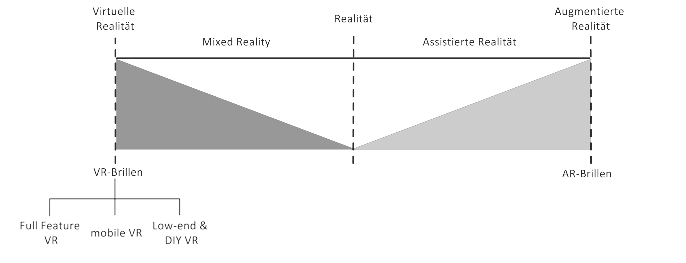
\includegraphics[width=1\textwidth]{data/bilder/VRvsAR.pdf}
    \caption{Einordnung von Smartglasses \cite[S.~28]{ThomasDirkMetzgerHelmutNiegemannHrsg2018}}
    \label{fig:Einordnung_Von_Smartglasses}
\end{figure}


\end{comment}
%
\subsection{Virtual Reality}
%
\emph{Virtual Reality (VR)} ist das völlige Ersetzen der wahrgenommenen Realität durch eine virtuelle Realität. Dabei wird dem Nutzer das Gefühl vermittelt, \enquote{Teil einer virtuellen Realität zu sein} \cite[S.~22]{ThomasDirkMetzgerHelmutNiegemannHrsg2018}. Virtual Reality-Brillen ermöglichen es dem Nutzer im Gegensatz zu Augmented Reality-Brillen komplett in eine virtuelle Realität zu wechseln. Realisiert wird dies durch vollständig geschlossene Gehäuse und Linsen, die vor dem Bildschirm befestigt sind. Mittels der Linsen vor dem Display wird ein scharfes Sehen in einem sehr nahen Bereich ermöglicht. Bei VR-Brillen wird zwischen Full-Feature, Mobile und Low-Budget VR-Brillen unterschieden. Full-Feature Brillen wie die Oculus Rift (Abbildung \ref{fig:OculusRift}) sind mit einer für jedes Auge separaten Full-HD-Auflösung mit hoher Bildwiederholungsrate ausgestattet und bieten dank einer leicht versetzten Anordnung einen dreidimensionalen Effekt. Mobile- und Low-Budget-VR-Brillen wie die Samsung Gear sind Produkte, die mithilfe eines aufgesetzten Smartphones eine Virtuelle Realität erstellen.
%
\begin{figure}[htbp]
    \centering
    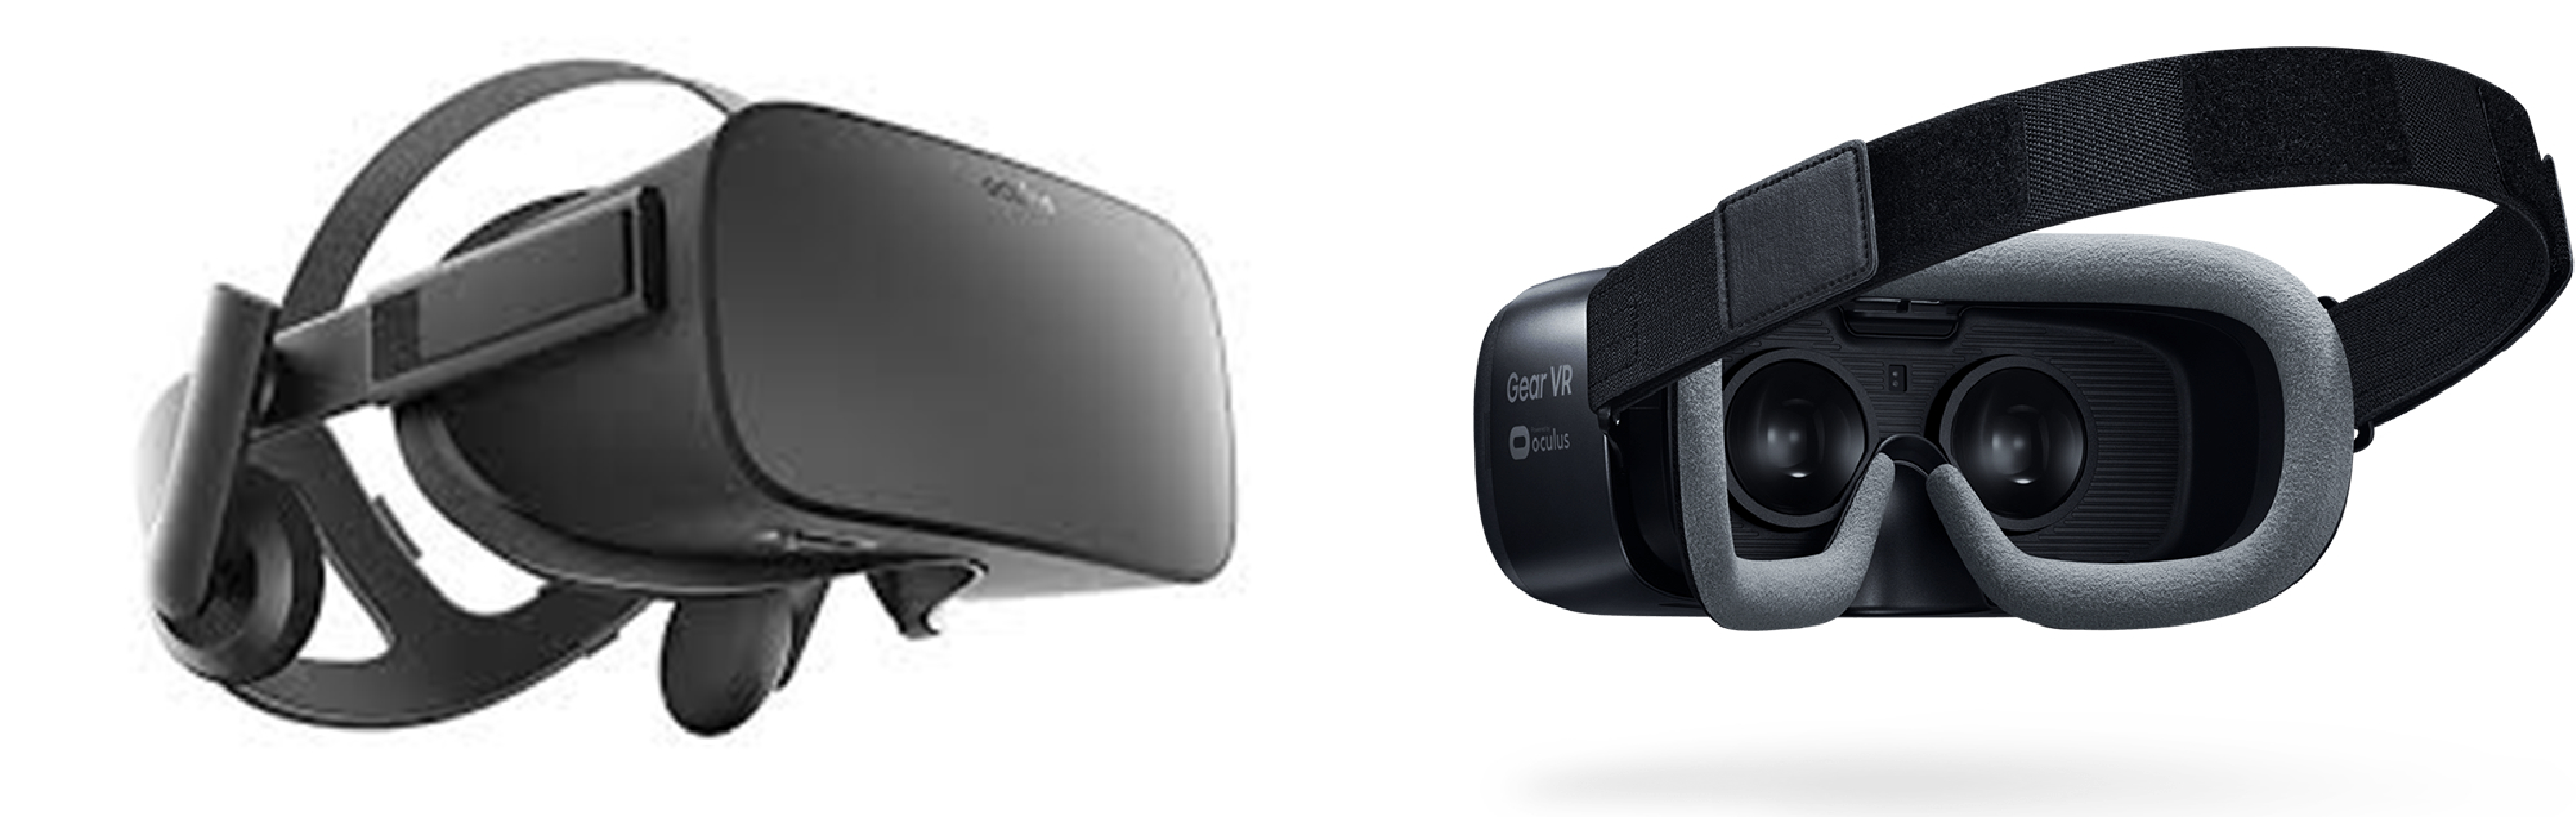
\includegraphics[width=1\textwidth]{data/bilder/Rift_Gear.pdf}
    \caption{Oculus Rift \cite{Oculus2018} (links) und Samsung Gear \cite{Samsung2018} (Rechts)}
    \label{fig:OculusRift}
\end{figure}
%

Der Anwender verliert durch diese Brillen das Gefühl, auf einen Bildschirm zu schauen. Die Außenwelt wird vollkommen ausgeblendet. Bewegungen mit dem Kopf werden automatisch in die virtuelle Welt übernommen. Nutzer bekommen das Gefühl, vollständig Teil der virtuellen Welt zu sein \cite[S.~22ff]{ThomasDirkMetzgerHelmutNiegemannHrsg2018}. 
%
\subsection{Augmented Reality}
%
\emph{Augmented Reality (AR)} ist im Gegensatz zu Virtual Reality das Einblenden von Informationen in das direkte Sichtfeld des Nutzers. Das Blickfeld des Trägers wird also um virtuelle Informationen erweitert \cite[S.~26]{Schwenke2016}. Es wird keine komplett virtuelle Realität erzeugt, sondern die reale Welt um digitale Inhalte ergänzt. Es gibt  unterschiedliche Arten von Brillen, die Augmented Reality-Effekte erzeugen. Differenziert wird zwischen Brillen, die \enquote{echte} Augmented Reality erzeugen und denen, die \emph{unterstützende Realität} erzeugen.

%
\subsubsection{Mixed Reality}
%
Unter \emph{Mixed Reality} wird eine Vermischung von realer Umgebung und virtueller Realität verstanden. Dabei wird eine Umgebung erstellt, in der reale und virtuelle Objekte kombiniert werden können. Objekte oder Personen der realen und virtuellen Welt können miteinander interagieren \cite{Schanze2017}. Diese Form der \enquote{echten} Augmented Reality wird durch Brillen wie die Microsoft Hololens erzeugt. Dabei werden kontextsensitive Informationen direkt im Sichtfeld des Nutzers eingeblendet. Oberflächenerkennung ermöglicht eine Verschmelzung von realer Welt und digitalen Informationen. Die Microsoft Hololens (Abbildung \ref{fig:Microsoft_Hololens}) beispielsweise ist in der Lage, dreidimensionale Hologramme im Sichtfeld des Nutzers anzuzeigen. Dies wird durch zwei transparente Displays ermöglicht. Diese völlige Manipulation der realen Welt wird auch als \emph{Mediated Reality} bezeichnet \cite[S.~46]{Schwenke2016}.
%
\begin{figure}[htbp]
    \centering
    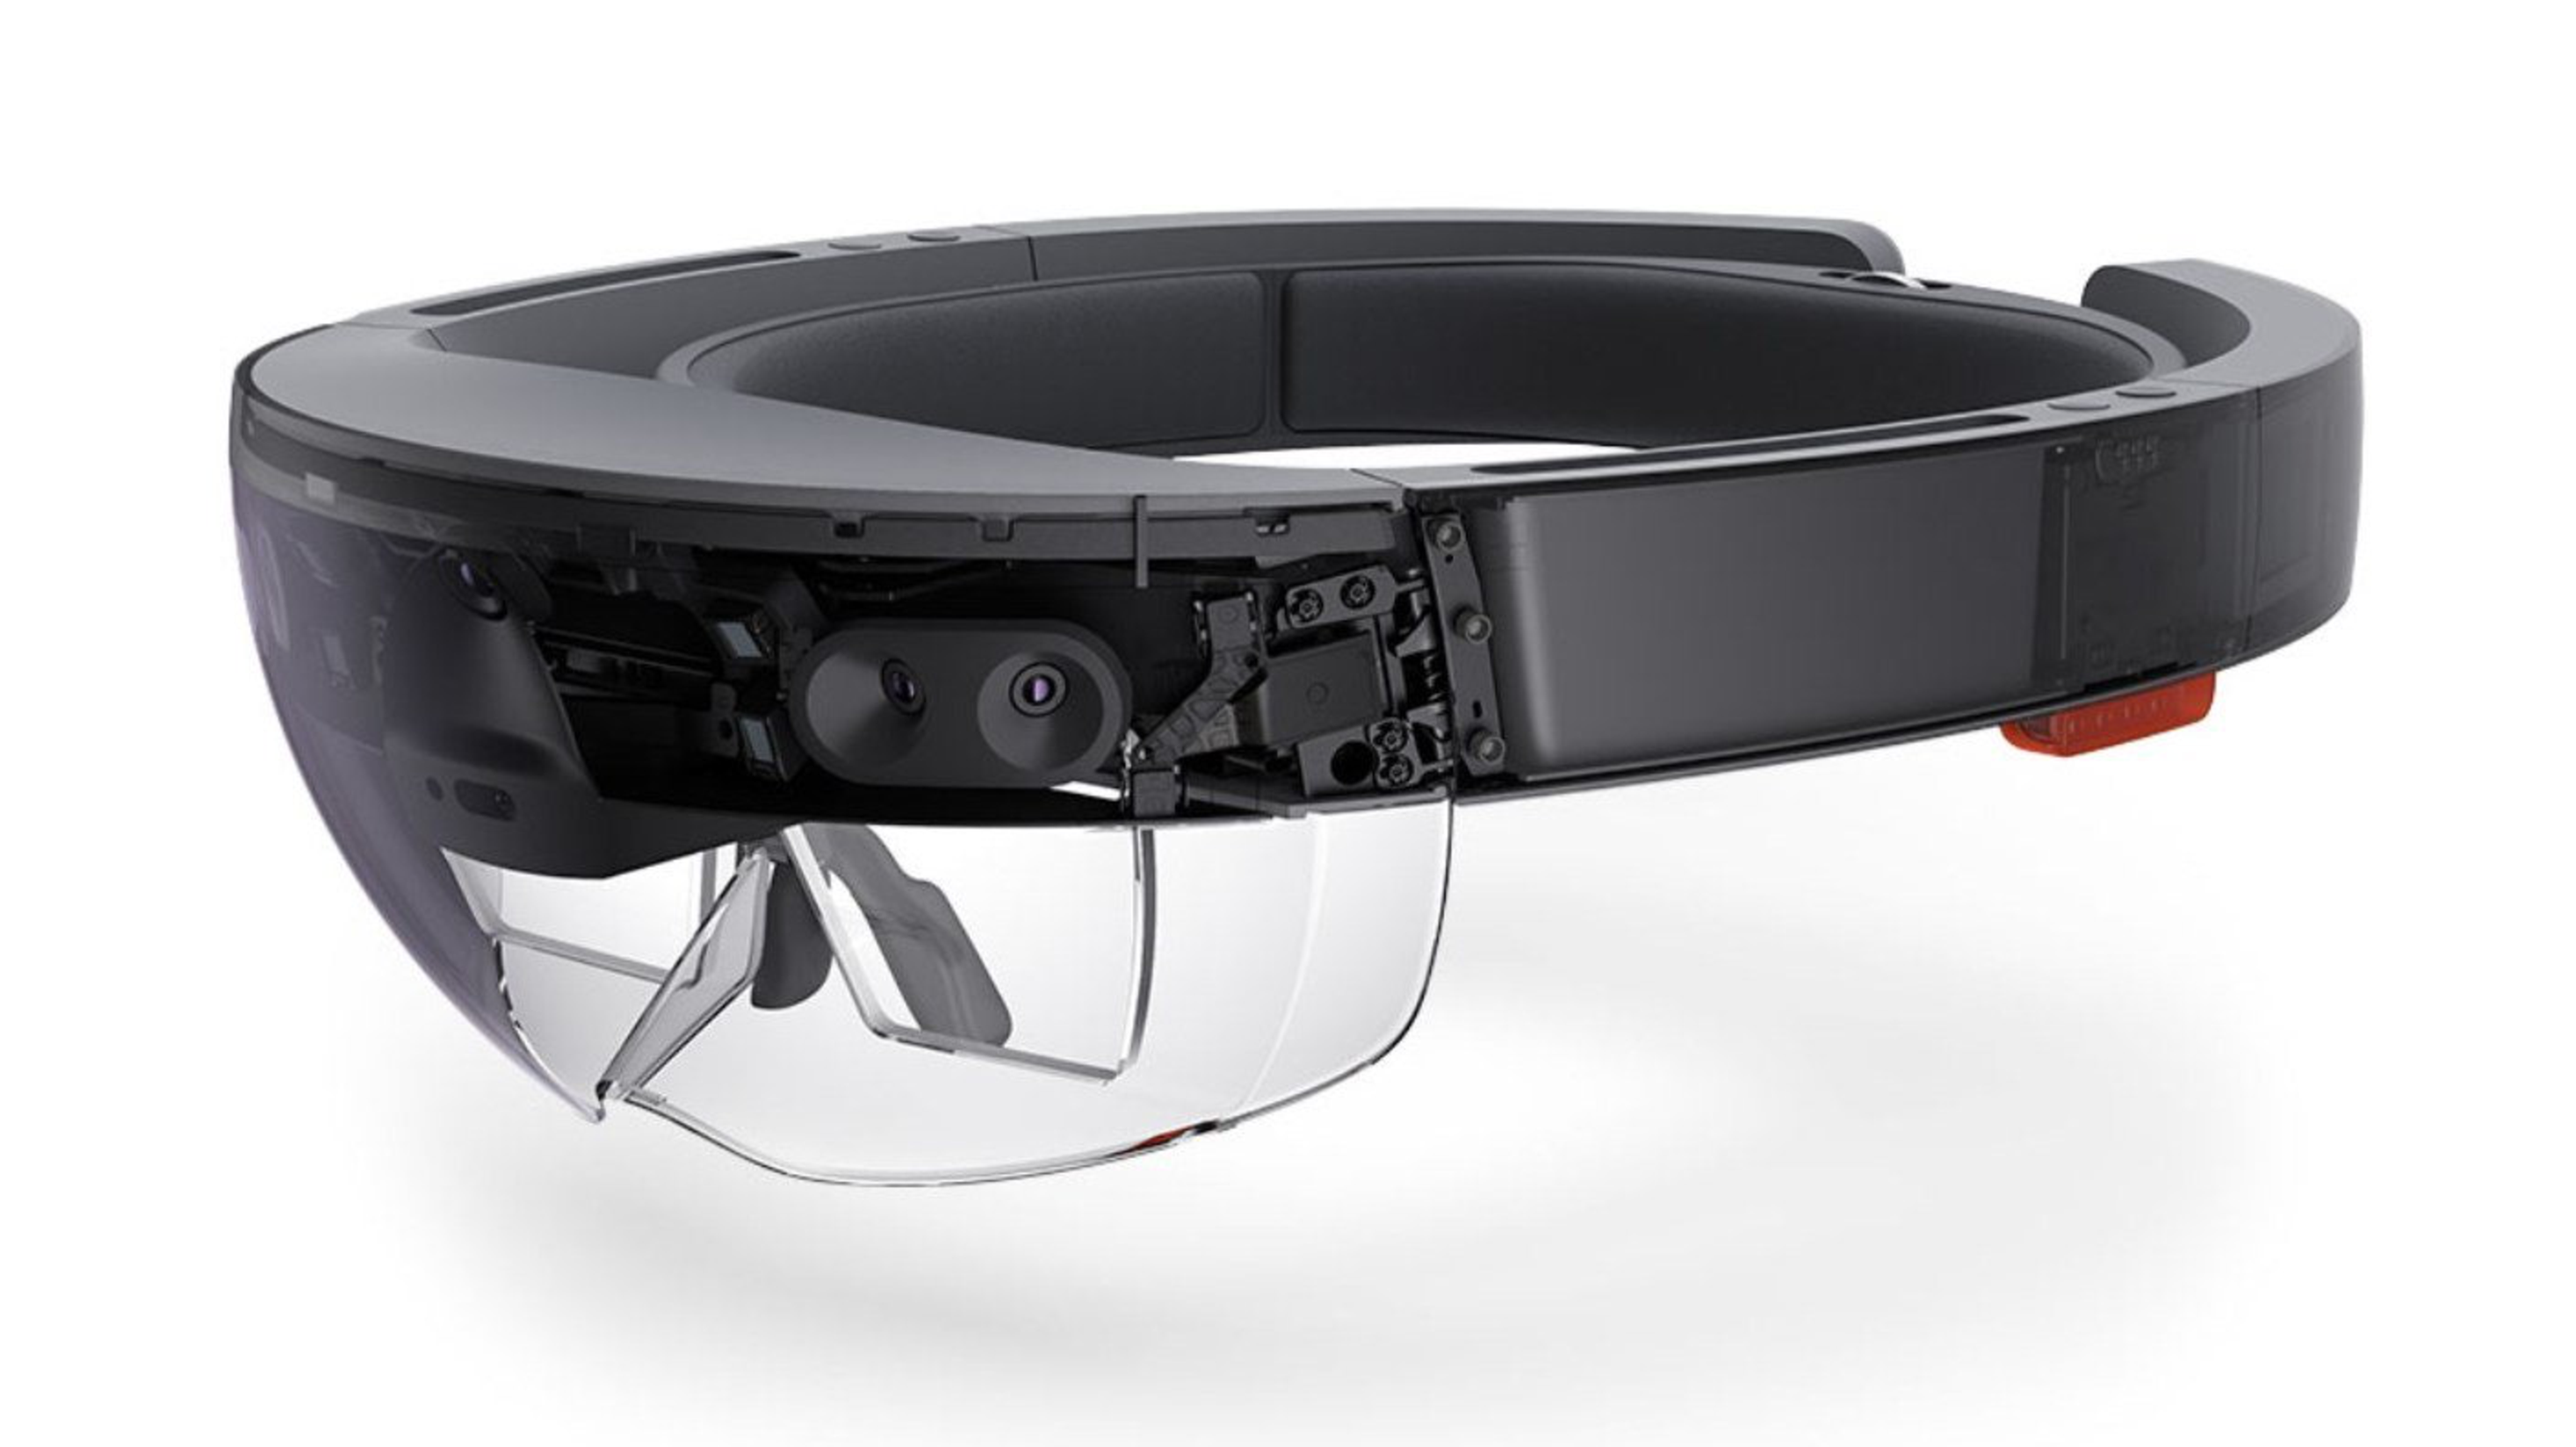
\includegraphics[width=0.5\textwidth]{data/bilder/Microsoft_Hololens.pdf}
    \caption{Microsoft Hololens \cite{O.V.}}
    \label{fig:Microsoft_Hololens}
\end{figure}
%
%

\subsubsection{Assistierte Realität}
\label{sec:AssistierteRealitaet}
%
Von \enquote{echter} AR abzugrenzen ist eine \emph{assistierte Realität}, die beispielsweise durch die \emph{Google Glass}, die \emph{Realwear hmt1} oder die \emph{Epson Moverio BT-200} (vgl. Kapitel \ref{sec:VergleichSmartglasses}) erzeugt wird.

Viele dieser Brillen werden mittels eines sogenannten \emph{Optical Head Mounted See-Through-Displays} \cite[S.~26]{Schwenke2016}, einem Prisma auf einem Auge, virtuelle Inhalte angezeigt, ohne Verlust der Realität mit sich zu ziehen. Bei manchen Assisted Reality-Brillen ist dieses Display jedoch nicht transparent. Es wird lediglich ein kleines Display vor dem Auge angeordnet (vgl. Realwear hmt-1, Kapitel \ref{sec:Realwear_hmt-1}). Im experimentellen Zustand befinden sich Geräte, die Informationen statt auf ein transparentes Display direkt auf die Retina des Auges projizieren \cite[S.~241]{Broll2013}. Ebenfalls zu erwähnen sind am Anfang ihrer Entwicklung befindliche Kontaktlinsen, sogenannte \emph{Smartlenses}, die Informationen mittels LEDs direkt auf die Kontaktlinse bzw. Netzhaut projizieren sollen \cite{Donath2014, Schwan2014}. Im medizinischen Bereich werden bereits heute sub-retinale Implantate getestet, die es ermöglichen, beschädigte Nerven zu ersetzen \cite{Young2013}. Dies ermöglicht ebenfalls die Einblendung von assistierten Realitäten.

Steuern lassen sich AR-Brillen mittels Objekterkennung durch die Kamera (bspw. Gestensteuerung) oder mobiler Hilfsmittel wie Headsets (\emph{Pick-by-Voice}) \cite{INTRALOGISTIK2016}. Es ist also möglich per Gesten- oder Sprachsteuerung zu navigieren. Manche Smartglasses besitzen zudem Touch-Sensoren.

Der Einsatz weiterer Sensoren, wie Trägheitssensoren oder Standortbestimmung sind ebenfalls möglich. Die Kamera einer solchen Smartglass kann zudem über weitere Sensoren, wie Termalsicht, verfügen \cite[S.~27]{Schwenke2016}. Oftmals sind diese Smartglasses mit WLAN, Mobilfunk oder Nahfeldtechnologien mit dem Internet verbunden oder über Schnittstellen mit einem externen Smartphone verknüpft, welches diese Funktionalitäten bereitstellt \cite[S.~28]{Schwenke2016}.

Für Augmented Reality sind Smartglasses zwar nicht zwingend erforderlich, da diese auch mittels bspw. Smartphones erreicht werden kann. So zeigt Apple mit dem AR-Kit \cite{Apple2018} die technischen Möglichkeiten mittels Augmented Reality in Smartphones. Es ist möglich mit dem Ende 2018 in iOS 12 erscheinenden AR-Kit 2 mit mehreren Nutzern in einer virtuellen über den realen Raum gelegten Realität zu interagieren. Smartglasses bieten jedoch viele Vorteile, da diese die Hände frei halten und die erweiterte Realität direkt vor den Augen des Betrachters und nicht in einem in der Hand befindlichen Smartphone dargestellt wird.

Softwaretechnische Beschränkungen der Smartglass sind grundsätzlich die gleichen, die auch für Android-Smartphones gelten. Auf allen gängigen Assisted Reality Smartglasses befindet sich als Betriebssystem Android (vgl. Kapitel \ref{sec:VergleichSmartglasses}). Weitere Beschränkung erfahren Smartglasses lediglich durch die geringe Displaygröße, die eine starke Anpassung einer Anwendung erfordert (siehe Kapitel \ref{sec:Grenzen_des_Einsatzes_von_Smartglasses}).
%
%
%
% - - - - - Vergleich verschiedener Smartglasses - - - - - - - - 
%
%
%
\section{Vergleich verschiedener Smartglasses}
\label{sec:VergleichSmartglasses}
% 2 Seiten
Da in dieser Arbeit Augmented Reality-Brillen und insbesondere Smartglasses mit assistierter Realität (\ref{sec:AssistierteRealitaet}) behandelt werden, werden im Folgenden einige Brillen dieses Bereiches vorgestellt.
%
%
%
% - - - - - - - - Google Glass - - - - - - - - - - - -
%
%
%
\subsection{Google Glass}
\label{sec:Google_Glass}
Der 2012 eingeführte Prototyp einer ersten Version von Google Glass (\enquote{Explorer Edition}) hat ein über dem rechten Auge plaziertes durchsichtiges quaderförmiges Display. Neben dem Display befindet sich eine hochauflösende Kamera sowie ein Mikrofon. Im Bügel der Brille ist die Recheneinheit angeordnet. Die Batterieleistung der Brille betrug beim ersten Prototypen nur wenige Stunden, ist in neueren Versionen jedoch deutlich erhöht worden \cite{Inc.2018}. Die Brille ist mit WLAN ausgestattet und ermöglicht mittels einer Verknüpfung mit einem Smartphone die Verbindung ins Mobilfunknetz sowie die Standortbestimmung mittels GPS.
%
\begin{figure}[htbp]
    \centering
    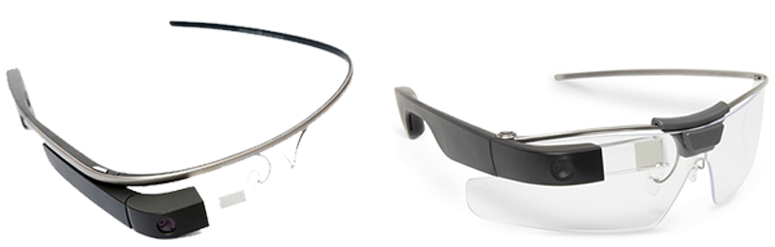
\includegraphics[width=0.8\textwidth]{data/bilder/Glass_1_und_2.png}
    \caption{Google Glass 1 (\enquote{Explorer Edition}) \cite{Reckmann2014a} (links) und Glass Enterprise Edition \cite{Huvelin2017} (rechts)}
    \label{fig:GlassModel}
\end{figure}
%

Die Brille lässt sich über verschiedene Sensoren steuern. So besitzt sie ein Touchpad im Bügel der Brille. Sprachbefehle ermöglichen ebenfalls die Steuerung der Brille. Augenbewegungen des Nutzers werden durch einen Infrarotsensor erfasst, sodass eine Auswahl von Elementen im User-Interface per Augensteuerung möglich ist. Die Kameraaktivität wird nicht angezeigt \cite[S.~30]{Schwenke2016}. Die Glass ist mit einem Android-Betriebssystem ausgestattet. Es gibt eine ausführliche Dokumentation mit speziellen APIs zur Entwicklung spezieller Glass-Anwendungen \cite{Google2018b}.

Mittlerweile hat Google eine speziell für den professionellen Einsatz optimierte Brille veröffentlicht, die \enquote{Glass Enterprise Edition} \cite{Inc.2018}. Diese Brille ist nur für den professionellen Einsatz zugelassen und wird nicht an Privatpersonen verkauft. 
%
%\insertMore{Unterschiede Glass Enterprise-Personal }
%
%
%
% - - - - - Epson Moverio BT-200 - - - - - - - - 
%
%
%
\subsection{Epson Moverio BT-200}
\label{sec:Epson_Moverio_BT-200}
Die Smartglass \emph{Moverio BT-200} von Epson hat im Gegensatz zur Google Glass zwei Bildschirme (je ein Bildschirm vor jedem Auge). 
%
\begin{figure}[htbp]
    \centering
    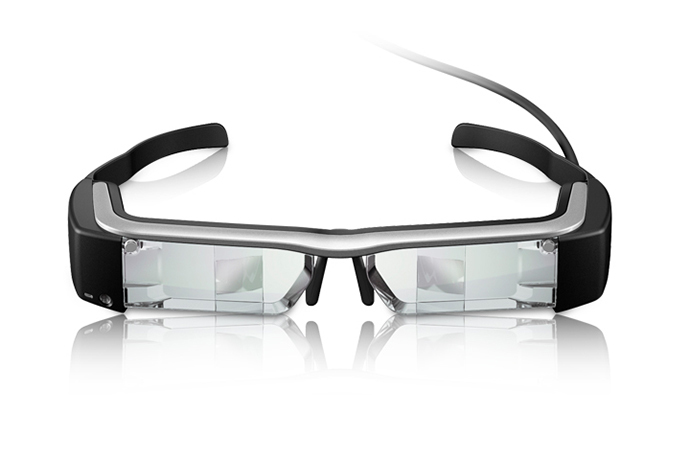
\includegraphics[width=0.4\textwidth]{data/bilder/Moverio_BT-200.png}
    \caption{Epson Moverio BT-200 \cite{Epson}}
    \label{fig:BT-200}
\end{figure}
%
Der Prozessor sowie die Batterie sind extern mittels eines Kabels mit der Brille verbunden. Die Brille verfügt über ein Touchpad, welches ähnlich dem der Google Glass am Bügel der Brille befestigt ist. Die Kamera der Brille ist deutlich geringer aufgelöst (640x480 Pixel), zeigt die Benutzung jedoch im Gegensatz zur Google Glass über eine kleine Leuchtdiode an. Wie auch bei der Google Glass ist das Betriebssystem der Moverio BT-200 Android \cite[S.~32]{Schwenke2016}. Diese Smartglass ist momentan nur in einer Developer-Edition erhältlich \cite{Epson}.
%
%
%
% - - - - - Vuzix M300 - - - - - - - - 
%
%
%
\subsection{Vuzix M300}
\label{sec:Vuzix_M300}
Die \emph{Vuzix M300} ist speziell für den professionellen Einsatz konzipiert. Sie verfügt über ein nicht-transparentes Display am rechten Auge, hat eine HD-Kamera und großen internen Speicher. Sie ist spritzwassergeschützt und nach Herstellerangaben robust gestaltet. Die Brille verfügt über ein Touch Pad sowie zwei Mikrofone zur Sprachsteuerung. 
%
\begin{figure}[htbp]
    \centering
    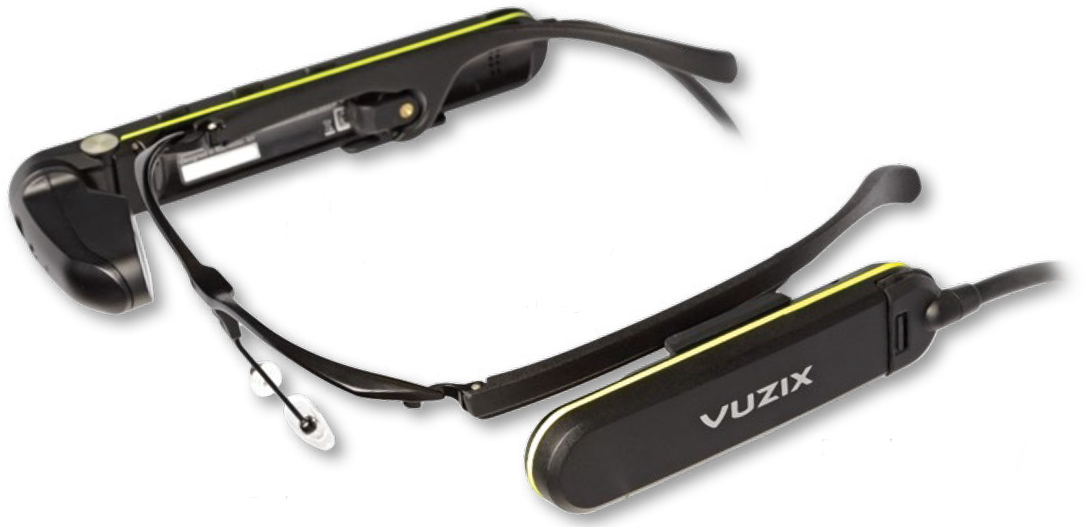
\includegraphics[width=0.4\textwidth]{data/bilder/m300-top.png}
    \caption{Vuzix M300 \cite{Vuzix2018}}
    \label{fig:Vuzix_M300}
\end{figure}
%

Die Vuzix M300 verfügt über schnell austauschbare Akkus, die je nach Anwendungszweck dynamisch angesteckt werden können. So gibt es je nach Anforderung verschieden schwere Akkus. Dies ermöglicht den Einsatz der Brille über einen beliebig langen Zeitraum.

Das Betriebssystem der Brille ist ebenfalls Android. Es lassen sich grundsätzlich alle für Android 6 konzipierten Apps auf der Brille bedienen, jedoch auch speziell für die Brille entwickelte Apps. Die Brille kann mit iOS- und Android-Smartphones gekoppelt werden, um Zugriff auf GPS und Mobilfunk zu erhalten. Zur Entwicklung für die App steht Entwicklern eine weitreichende Dokumentation sowie spezielle APIs zur Verfügung. \cite{Vuzix2018}
%
%
%
% - - - - - Realwear hmt-1 - - - - - - - - 
%
%
%
\subsection{Realwear hmt-1}
\label{sec:Realwear_hmt-1}
%
\begin{figure}[htbp]
    \centering
    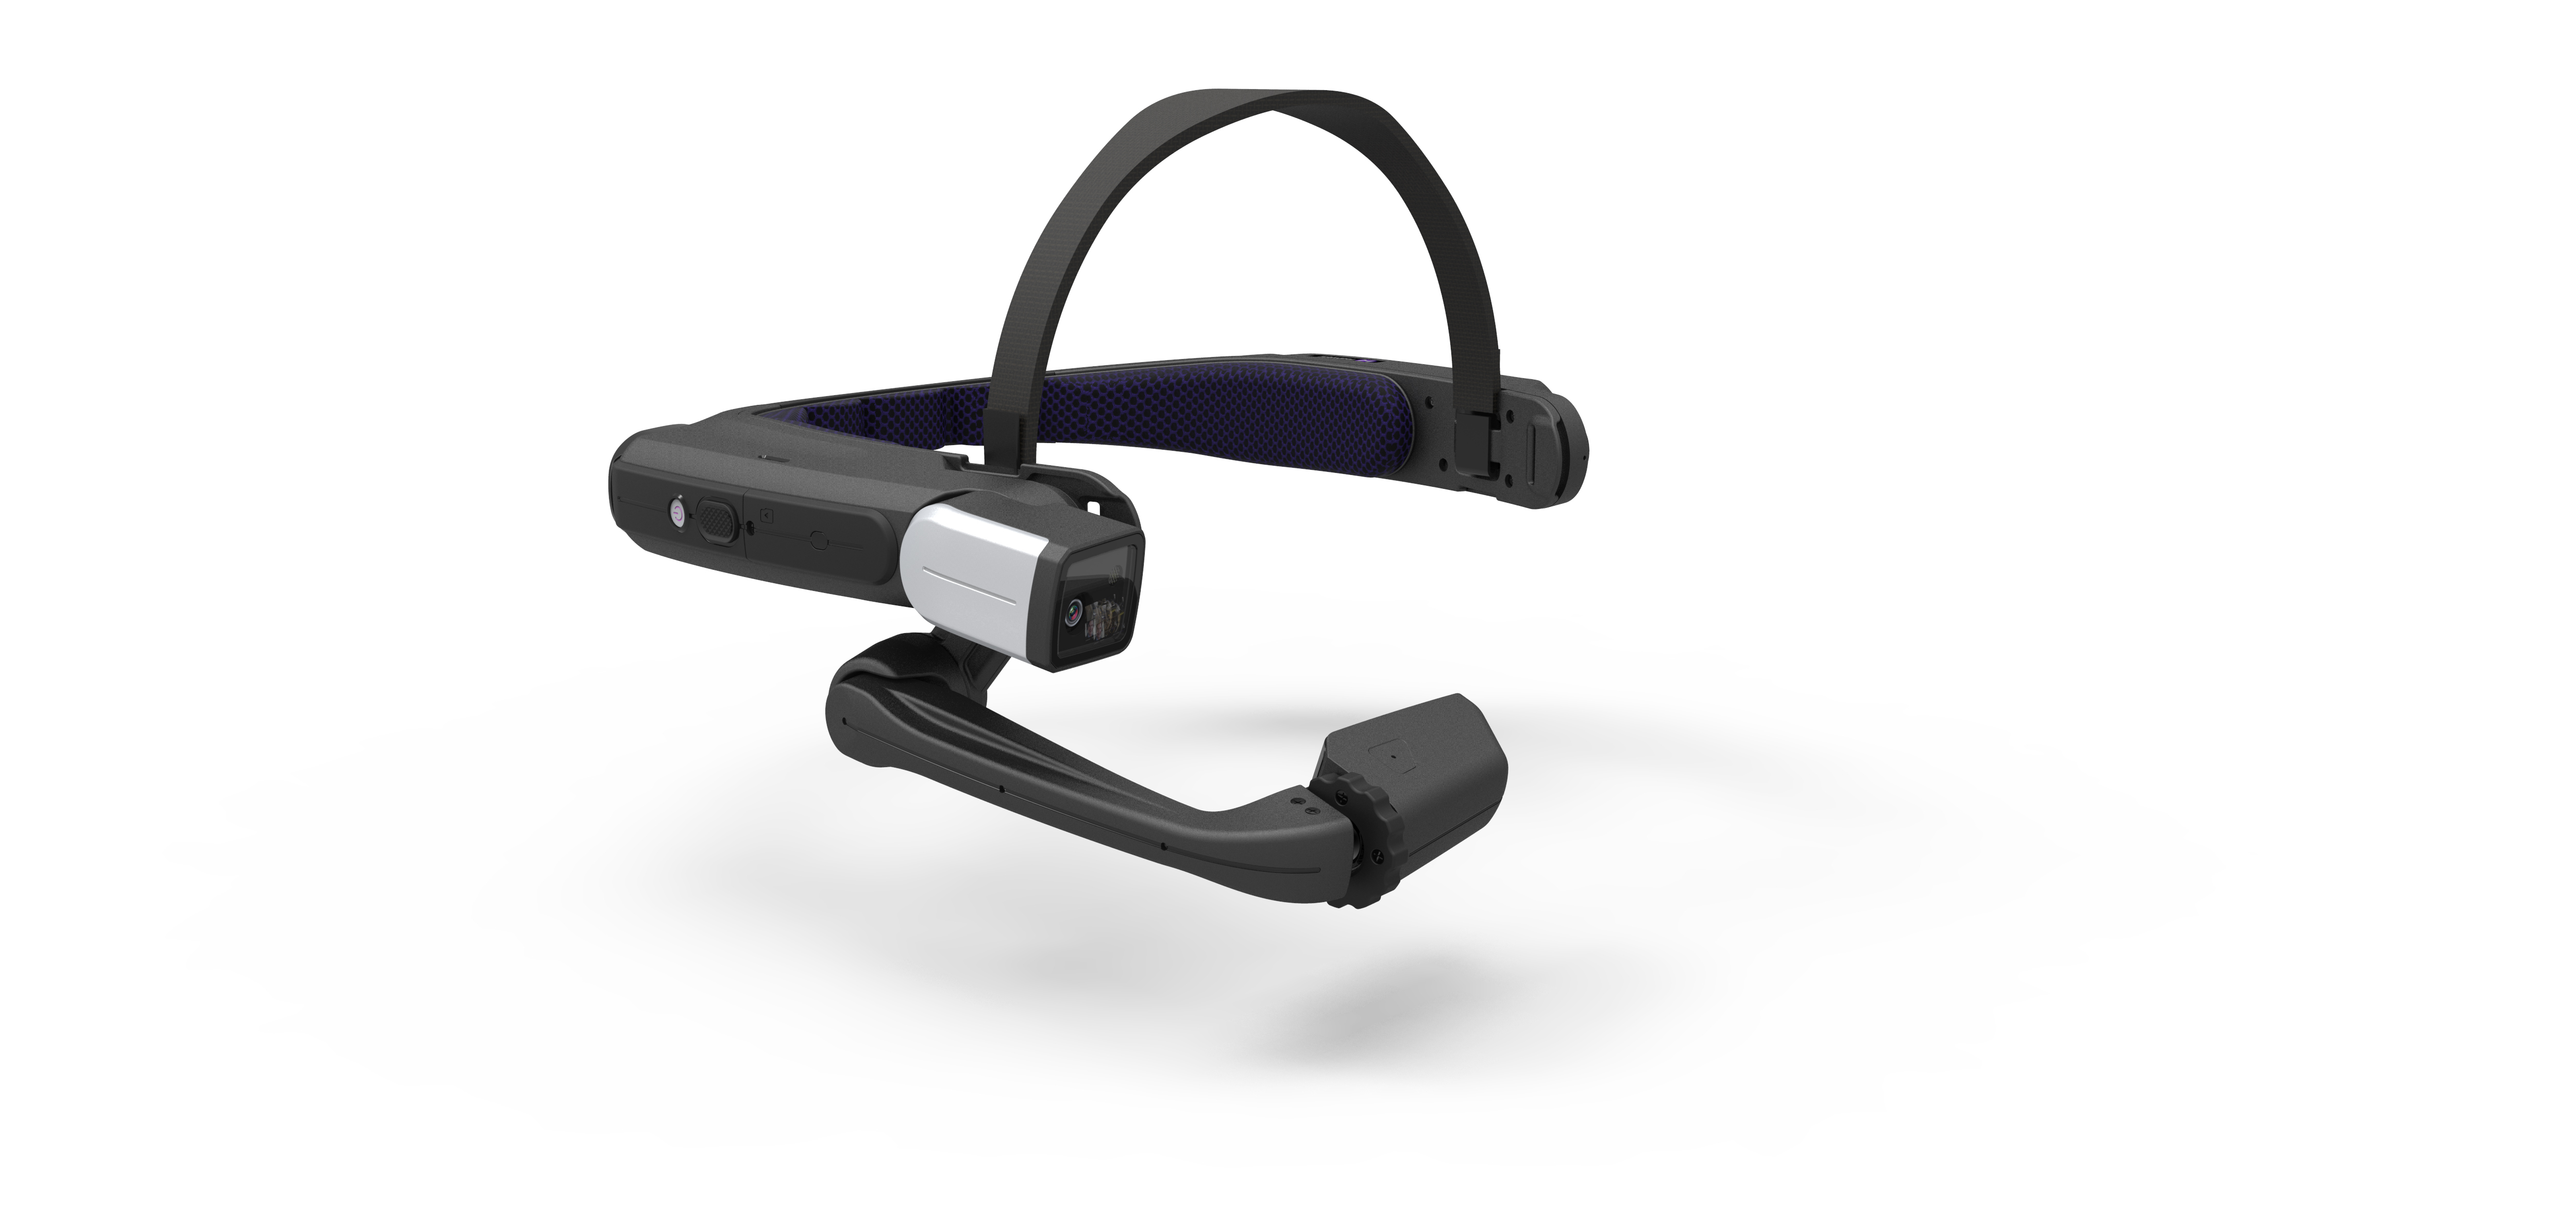
\includegraphics[width=0.9\textwidth]{data/bilder/HMT_1.jpg}
    \caption{Realwear hmt-1 \cite{Wire2017}}
    \label{fig:hmt1}
\end{figure}
%

Die \emph{Realwear hmt-1} ist ebenfalls für den professionellen Einsatz optimiert. Ähnlich der Google Glass ist ein Display über dem rechten Auge befestigt. Dazu kann der Bügel mit dem Display sowohl über dem linken wie auch dem rechten Auge befestigt werden.

Im Gegensatz zur Glass ist dieses Display jedoch nicht transparent, es ist jedoch für den Außeneinsatz konzipiert und ist auch bei starkem Sonnenlicht nutzbar. Die Brille ist vollständig abwischbar. Sie erfüllt dazu den IP66-Standard \cite{Realwear2018}.

Prozessor und Batterie sind im Bügel der Brille befestigt. Die Brille  besitzt eine Sprachsteuerung mit integrierter Noice-Cancellation mittels vier eingebauter Mikrofone. Die Batterie der Brille hält einen gesamten Arbeitstag. Im Gegensatz zur Glass und BT-200 ist die hmt-1 so ausgelegt, dass sie Stürze aus 2~m Höhe auf Betonboden übersteht. Wie auch Glass und BT-200 ist das Betriebssystem der hmt-1 Android. Es gibt eine gut dokumentierte Entwicklerdokumentation und APIs zur Entwicklung von speziell für die Brille konzipierten Android-Anwendungen \cite{Realwear2018}.
%
%
%
% - - - - - Smartglasses im beruflichen Umfeld - - - - - - - - 
%
%
%
\section{Smartglasses im beruflichen Umfeld}
\label{sec:Smartglasses_im beruflichen_Umfeld}
% 3 Seiten
Die Logistikbranche ist Deutschlands drittgrößte Branche \cite{Zobel2016}. In der Logistikbranche werden Datenbrillen in Form von Assistierten AR-Brillen eingesetzt \cite{Niemoller2017}.
\\
Smartglasses ermöglichen die Digtialisierung von Arbeitsprozessen und machen es möglich, die Integration von Mitarbeitern in Unternehmensprozesse zu verbessern \cite{Zobel2016}. Sie liefern kontextabhängige Informationen, beispielsweise durch das Einlesen von Barcodes bzw. QR-Codes. Angestellte der Logistikbranche der Transportlogistik werden so in Echtzeit mit Informationen, wie beispielsweise Lieferaufträgen versorgt. In einer Use-Case-Studie von Niemöller \cite{Niemoller2017} wurden insgesamt 36 Einsatzmöglichkeiten für Smartglasses im Logistikdienstleistungssektor ermittelt. Die relevantesten Use-Cases werden im Folgenden dargestellt:
\\
Zum einen wurde das Themenfeld Kommunikation herausgearbeitet. Mittels Smartglasses ist das Anzeigen von Handlungsanweisungen sowie die Darstellung von Videoinformationen mittels Streaming oder Offlinevideos möglich. Eine vereinfachte Kommunikation durch die Übersetzung von Texten ist ebenso möglich. Im Themenfeld Qualitätssicherung ist eine automatisierte Kontrolle mittels einer kamerabasierter Fehlererkennung sowie entsprechender Rückmeldung an den Nutzer möglich. Das Haupteinsatzfeld ist jedoch die Identifizierung anhand gespeicherter Merkmale wie Farbe, Größe und Geometrie oder auch durch die Identifizierung mittels Bar- und QR-Codes \cite{Niemoller2017}. Identifizierung von Objekten ermöglicht die Anzeige von Zusatzinformationen. Im Themenfeld Sicherheit ist die kontextabhängige Darstellung von Sicherheits- und Warnhinweisen möglich. 

Auf dem Fachkongress \emph{Smart Glasses Experience Days} \cite{Manokaran-Pathamathan2017} wurden weitere Einsatzfelder aufgezeigt. So können über die Datenbrille Montage- oder Reparaturanleitungen angezeigt werden. Zwecks Dokumentation werden Arbeitsschritte und Informationen des vorhergehenden Angestellten angezeigt. Per Remoteunterstützung können Angestellte Hilfe bei komplizierten Arbeitsschritten erhalten. Für Lagermitarbeiter können Anweisungen angezeigt werden, wie und in welcher Reihenfolge Anweisungen befolgt werden sollen.

Neben der Logistikbranche werden Smartglasses auch in anderen Branchen eingesetzt. In dem Studienbericht \emph{Smart Glasses in der Produktion} des Fraunhofer-Instituts für Produktionstechnologie IPT von 2016 \cite{Plutz} wurde der Einsatz von Smartglasses im beruflichen Umfeld der industriellen Produktion analysiert. So setzen 3,4\% der 237 befragten Unternehmen  Smartglasses bereits ein. 15,1\% wollen diese in nächster Zeit einsetzen. Die häufigsten Anwendungsgebiete waren Mitarbeiterschulungen (27,3\%), Fernwartung/Videotelefonie (27,1\%), Echtzeitanzeige von Informationen (22,8\%) und industrielle Bildverarbeitung (17,5\%). Laut dem Bericht ist es möglich, nicht nur prozessrelevante Informationen zur Verfügung zu stellen, sondern Angestellte auch dazu zu befähigen, Informationen prozessintegriert zu erzeugen. Zudem sei es möglich, hoch aufgelöste Zeiterfassung manueller Tätigkeiten zu realisieren und Prüfdaten nicht wie bislang handschriftlich zu erfassen, sondern dabei die Hände frei zu haben.

Laut einer Pressemitteilung des Logistikunternehmens DHL vom 2. August 2017 führt der Einsatz von Smartglasses zu einer 15-prozentigen Produktivitätssteigerung bei geringerer Fehlerquote \cite{DeutschePostDHLGroup2017}. Mittels Sprachsteuerung lassen sich einzelne Kommissionieraufträge aufrufen und die nötigen Informationen auf dem Display anzeigen. So ist es möglich, Lagerort, Lagerplatz und die zu packende Anzahl der Ware anzuzeigen statt wie bisher auf papierbasierte Auftragsanweisungen zurückzugreifen. 

Das Unternehmen Bosch setzt in ihrer Logistiksparte ebenfalls Smartglasses ein. Für Bosch ist vor allem die Tatsache von Vorteil, dass die Angestellten beim Scannen von Barcodes und QR-Codes freihändig agieren können \cite{Spinger2014}. 
%
\chapter{Anforderungsanalyse}
\section{Ablauf der Medizinprodukteaufbereitung}
\section{Anforderungen bei der Medizinprodukteaufbereitung}
\section{Smartglasses im Bereich der Medizinprodukteaufbereitung}
\subsection{Einsatzmöglichkeiten}
\subsection{Spezifische Anforderungen an Smartglasses im Bereich der Medizinprodukteaufbereitung}
\subsection{Datenschutz}
\subsection{Arbeitssicherheit}
\subsection{Grenzen des Einsatzes von Smartglasses}

%
\chapter{Konzept}
% 0,5 Seiten
%
% - - - - - - - - - - - - - - - - - - - - - - - - 
%
\section{Interaktionsmöglichkeiten}
% 2 Seiten
%
% - - - - - - - - - - - - - - - - - - - - - - - - 
%
\section{Objekterkennung}
% 2 Seiten 
%
% - - - - - - - - - - - - - - - - - - - - - - - - 
%
\subsection{Externe Peripherie}
% 1 Seite 
%
% - - - - - - - - - - - - - - - - - - - - - - - - 
%
\subsection{Medienverwaltung}
% 2 Seiten 
%
% - - - - - - - - - - - - - - - - - - - - - - - - 
%
\section{Medienpräsentation}
% 2 Seiten
%
% - - - - - - - - - - - - - - - - - - - - - - - - 
%
\section{Medienerfassung/-erstellung}
% 2 Seiten
%
%
%
%
% - - - - - Prototyp - - - - - - - - 
%
%
%
\chapter{Prototyp zur Unterstützung in der Sterilgutversorgung}
\label{ch:Prototyp}
In dieser Arbeit wurde ein Prototyp für die \emph{Realwear hmt-1} implementiert. Die Funktionalität, verwendete Technologien sowie die Implementation werden im Folgenden vorgestellt.
%
%
%
% - - - - - Funktionalität des Prototypen - - - - - - - -
%
%
%
\section{Funktionalität des Prototypen}
Mithilfe des Prototypen sind zwei grundsätzliche Funktionalitäten möglich. Es ist einerseits möglich, aus einer bestehenden Liste von Bildergalerien eine Galerie auszuwählen und anzuzeigen. Andererseits kann eine Slideshow in Form einer JSON-Datei per QR-Code von einem Server geladen werden. Innerhalb der Bildergalerie ist es dann möglich, vor und zurück zu navigieren. 
Slideshowauswahl und Slides sind in einer Listenansicht dargestellt, die es ermöglicht, stets 4-5 Elemente auf einmal anzuzeigen und bei Bedarf weitere Elemente nachzuladen. Dies wird mit einem Vor- und einem Zurückbutton realisiert.

Die andere Hauptfunktionalität betrifft Videos. Es ist möglich,  Videos aufzuzeichnen und dieses abzuspielen. Es ist ebenso möglich, einen QR-Code mit einer Adresse auf ein MP4-Video aufzurufen und dieses Video zu streamen. Innerhalb eines abgespielten Videos ist es möglich, 10 Sekunden vor oder zurück zu spulen und zu pausieren. Zudem ist es möglich, Kapitelmarken zu setzen und in einer eigenen Ansicht zu bearbeiten.

All diese Funktionalitäten können via Sprachsteuerung ausgewählt werden. Dazu müssen die Beschriftungen der Buttons laut vorgelesen werden. Die Brille interpretiert dann diese Eingaben als \emph{Click}-Events und ruft entsprechende Funktionen auf.

In der Praxis können Bilder-Slideshow und Videos eingesetzt werden, um Angestellten der AEMP wichtige Informationen zu medizinischen Instrumenten zu geben. So können Hyperlinks zu Anleitungen per QR-Code oder Barcode auf die Smartglass geladen werden und von einem externen Server gestreamt werden.

Um auch ohne Internetverbindung arbeiten zu können, ist es zu Beginn des Appstarts möglich, eine lokale Server-URL per QR-Code einzulesen. Diese wird anschließend vor alle per QR-Code eingelesenen URLs gesetzt, sodass es möglich ist auch in einer Umgebung wie der AEMP, in der keine Internetverbindung zur Verfügung steht, auf Videos und Bilder eines lokalen Servers zuzugreifen. 

Zum Testen wurde ein lokaler NodeJS-Server aufgesetzt, welcher Mediendaten ausliefert.
%
%
%
% - - - - - Verwendete Technologien - - - - - - - - 
%
%
%
\section{Verwendete Technologien}
\label{sec:Verwendete_Technologien}
% 3 Seiten
Für die Implementierung des Prototypen wurde \emph{Android Studio} mit Android in Version 23 verwendet, da dies die neueste Version ist, die von der \emph{hmt-1} unterstützt wird. Die API der \emph{hmt-1} ermöglicht den Zugriff auf die Hardwarefunktionalitäten sowie auf die Sprachsteuerung der Smartglass. Mittels eines Eintrags \emph{\enquote{android:contentDescription}} können Sprachbefehle zu beliebigen Elementen hinzugefügt werden. Die Elemente reagieren dann auf den im Eintrag angegebenen Sprachbefehl und lösen ein \emph{Click}-Ereignis aus.

Die API der Smartglass hat zudem eine Funktionalität, um Barcodes und QR-Codes auszulesen und den Inhalt zurückzugeben und eine API, um Videos in hoher Auflösung aufzuzeichnen. 

Der Prototyp speichert aufgezeichnete Videos auf dem Gerät und serialisiert das dazugehörige Datenobjekt (vgl. Kapitel \ref{sec:Datenmodell}) auf dem Gerätespeicher. Externe Videos und Bilder werden per JSON-Objekt, welches über einen Link von einem Server geladen wird, geladen. Diese JSON-Objekte enthalten alle notwendigen Informationen. So enthält das JSON-Objekt der Slideshow ein Array aus Objekten mit Namen und URL. Beim Video wird der Name, die URL und die Kapitel mit Namen und Position in Millisekunden gespeichert (vgl. Listing \ref{lst:json_video} und \ref{lst:json_slides}).

Der verwendete lokale Server ist ein NodeJs-Server, welcher über die IP-Adresse und den verwendeten Port einen Ordner auf dem Dateisystem freigibt.
%
%
%
% - - - - - Implementation - - - - - - - - 
%
%
%
\section{Implementierung}
\label{sec:Implementation}
Im Folgenden wird die Implementierung des Prototypen beschrieben. 

Das Programm folgt bei der Videofunktionalität dem Model-View-Controller (\emph{MVC})- Pattern, bei dem eine Trennung von Programmlogik, Model und View eingehalten wird.
%
%
%
% - - - - - User-Interface - - - - - - - - 
%
%
%
\subsection{User-Interface (View)}
Die Android-Anwendung wurde nach dem in Abbildung \ref{fig:Storyboard_des_Prototypen} gezeigten Storyboard erstellt. Die Anwendung beginnt in einem Hauptmenü, welches ermöglicht, per Sprachbefehl einen von zwei Buttons auszuwählen. Mit dem ersten Button wird der Nutzer zur Slideshow-Seite weitergeleitet. Beim zweiten Button wird auf die Videoanzeige und beim dritten Button auf die Video-Aufzeichnen Funktion weitergeleitet. Mittels eines \enquote{Schritt-Zurück-Befehls} der Smartglass wird der androidtypische \enquote{Zurückbefehl} betätigt.

\begin{figure}[htbp]
    \centering
    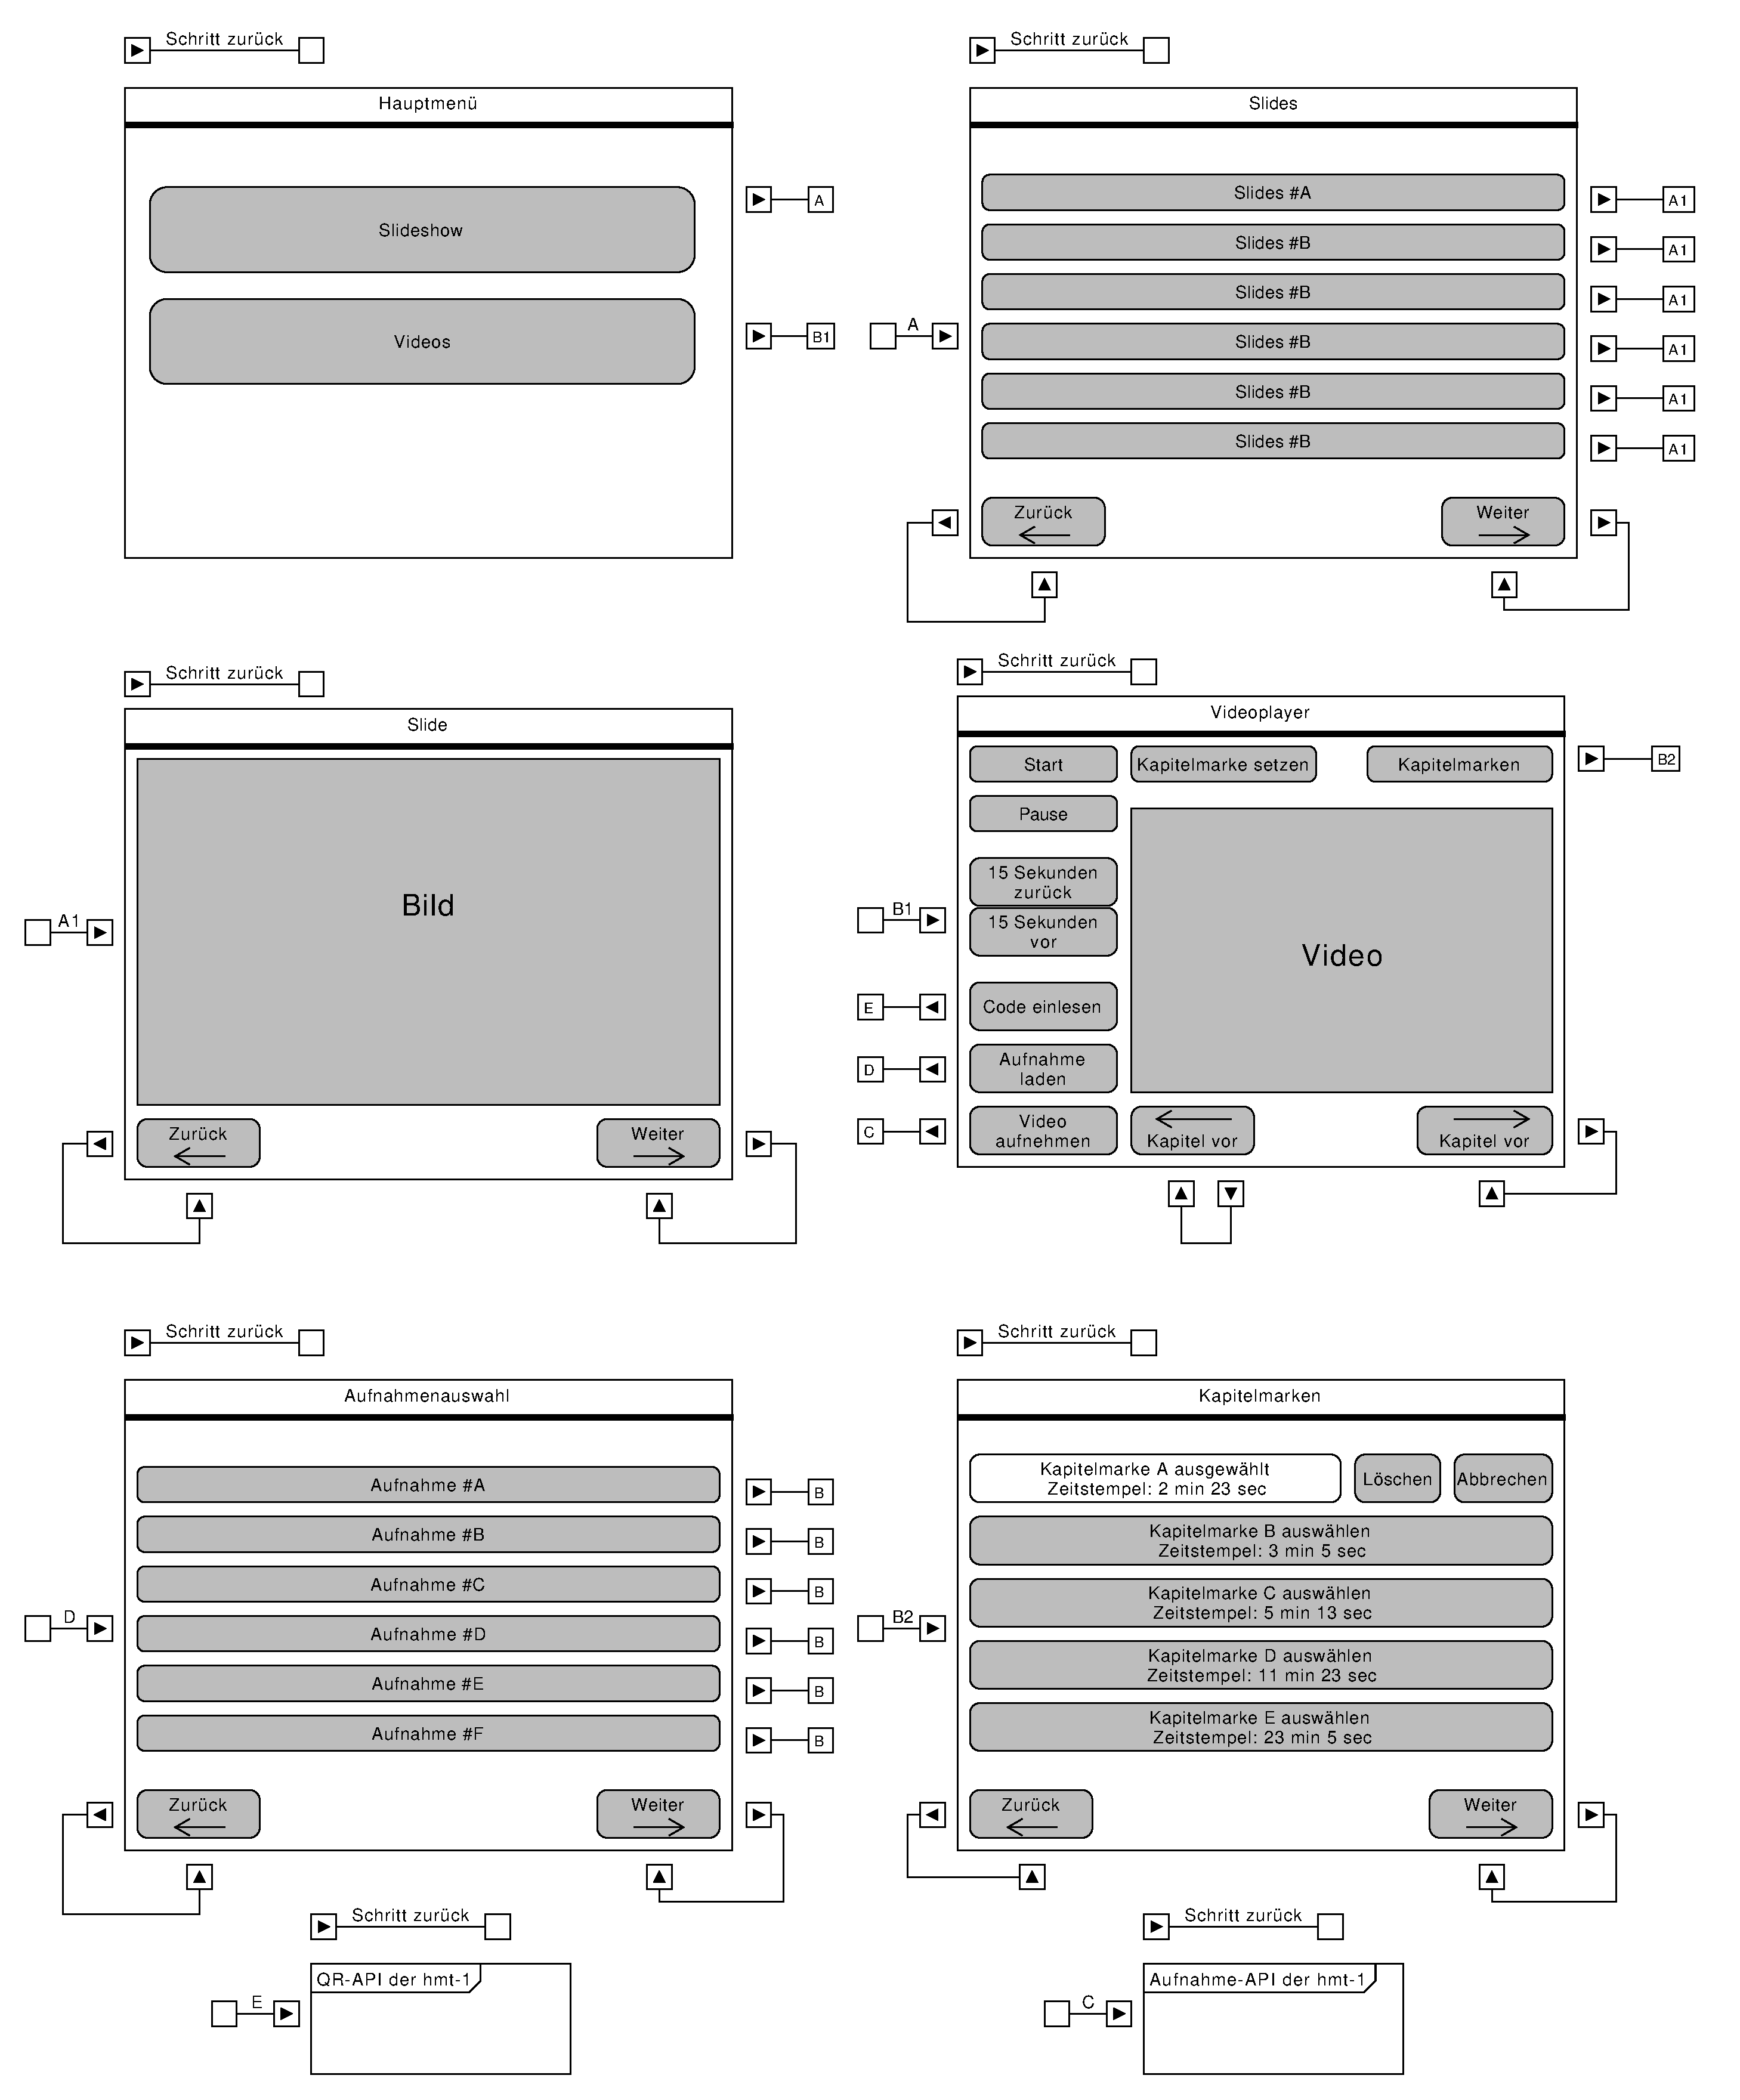
\includegraphics[width=1\textwidth]{data/bilder/UI-Storyboard.pdf}
    \caption{Storyboard des Prototypen}
    \label{fig:Storyboard_des_Prototypen}
\end{figure}

Die Slideshow besteht aus zwei Ansichtstypen. In der ersten Ansicht, welche über das Hauptmenü erreichbar ist, wird eine Liste von Buttons angezeigt, über die einzelne Slides ausgewählt werden können. Am unteren Rand des Fensters ist ein \enquote{Weiterbutton}, welcher die Liste der Buttons aktualisiert, um weitere Slides zur Auswahl zu stellen. Dies ist notwendig, da bei der \emph{hmt-1} klassisches scrollen durch eine Liste nicht möglich ist. Es ist lediglich das Scrollen durch eine kurze Liste per Kopfgesten möglich.

Über einen Button \enquote{Code einlesen} ist es möglich, einen QR-Code zu lesen, der einen Link zu einer JSON-codierten Slideliste kapselt und es so ermöglicht, die Slides dynamisch nachzuladen.

Wird eine Bilderliste ausgewählt, so wird auf eine Unterview verlinkt. Diese besteht aus einer \emph{Image-View} sowie zwei Buttons: \enquote{vorwärts} und \enquote{zurück}. Im Bild wird das aktuelle Bild der Bilderliste angezeigt. Mit \enquote{weiter} wird das nächste, mit \enquote{zurück} das vorherige Bild angezeigt.

Aus der Haupt-Einstiegsview kann zudem die \emph{Videoplayer}-View geöffnet werden. Diese Ansicht besteht aus zwei Bereichen. Links ist eine Sammlung von insgesamt 7 Buttons zum starten und stoppen, vor- bzw. zurückspulen des Videos um 10 Sekunden, Einlesen eines QR-Codes und Einlesen des Videolinks in den Videoplayer. Diese Buttons werden dynamisch ein- bzw ausgeblendet, je nach Stadium, in dem die App sich befindet. So werden immer nur die Buttons angezeigt, die wirklich verwendet werden können. Zusätzlich sind noch zwei Buttons zum Aufnehmen eines Videos und zum Laden einer Aufnahme in den Player. Rechts ist ein Videofenster angebracht, in dem die Videos angezeigt werden.

Einlesen des QR-Codes sowie die Aufnahme des Videos werden mithilfe der API der \emph{hmt-1} realisiert. Der eingelesene Link enthält ein JSON-Objekt, welches den Link sowie die Kapitel enthält. Das Ergebnis wird in der View angezeigt.

Ist ein Video geladen, so werden die Buttons zur Bearbeitung und Verwendung der Kapitelmarken sichtbar. Mittels zweier Buttons an der unteren Bildschirmseite ist es möglich, die jeweils nächsten und vorherigen Kapitelmarken anzusteuern. Mit einem Button an der oberen Bildschirmhälfte ist es möglich, eigene Kapitelmarken an der aktuellen Position des Videos zu setzen. Diese können mittels Spracheingabe benannt werden.

Wird ein Button \enquote{Kapitel} aufgerufen, so wird eine eigene View zur Verwaltung von Kapitelmarken angezeigt, die ähnlich der Slideshowauswahl funktoniert. Hier wird eine Liste angezeigt, in der alle Kapitel aufgelistet werden. Wählt der Nutzer ein Kapitel aus, so erscheinen \enquote{Löschen}- und \enquote{Abbrechen}-Buttons. Mittels \enquote{Löschen} kann das ausgewählte Kapitel gelöscht werden. 
%
%
%
% - - - - - Datenmodell - - - - - - - - 
%
%
%
\subsection{Datenmodell (Model)}
\label{sec:Datenmodell}
In Abbildung \ref{fig:Klassendiagramm} ist neben der Klassenstruktur des Controllers das Klassendiagramm des Models gezeigt. Dieses besteht aus insgesamt vier Klassen: den Basisdatentypen \enquote{Slide}, \enquote{Video} sowie \enquote{VideoChapter} und der Liste von Slides \enquote{SlideList}. 

Die Klasse \enquote{Slide} kapselt einen String \enquote{fileURL} und den Titel \enquote{title}. 
Die Klasse \enquote{VideoChapter} dient zur Speicherung eines Kapitels eines Videos und wird von der Klasse Video verwendet. Ein VideoChapter besteht aus einer Ganzzahl \enquote{position} und dem Namen des Kapitels als String. Die Klasse \enquote{SlideList} kapselt eine \emph{ArrayList} von Slides sowie den Namen der SlideList.
Die Klasse \enquote{Video} besteht aus dem Namen der Datei, in welcher das Video im Dateisystem gespeichert wird, der URL des Videos, dem Titel, sowie aus einer ArrayList von VideoChapter. Video besitzt zudem öffentliche Methoden zum Hinzufügen und Entfernen von Kapiteln sowie zum Persistieren und laden des Video-Models im Dateisystem.
\begin{figure}[htbp]
    \centering
    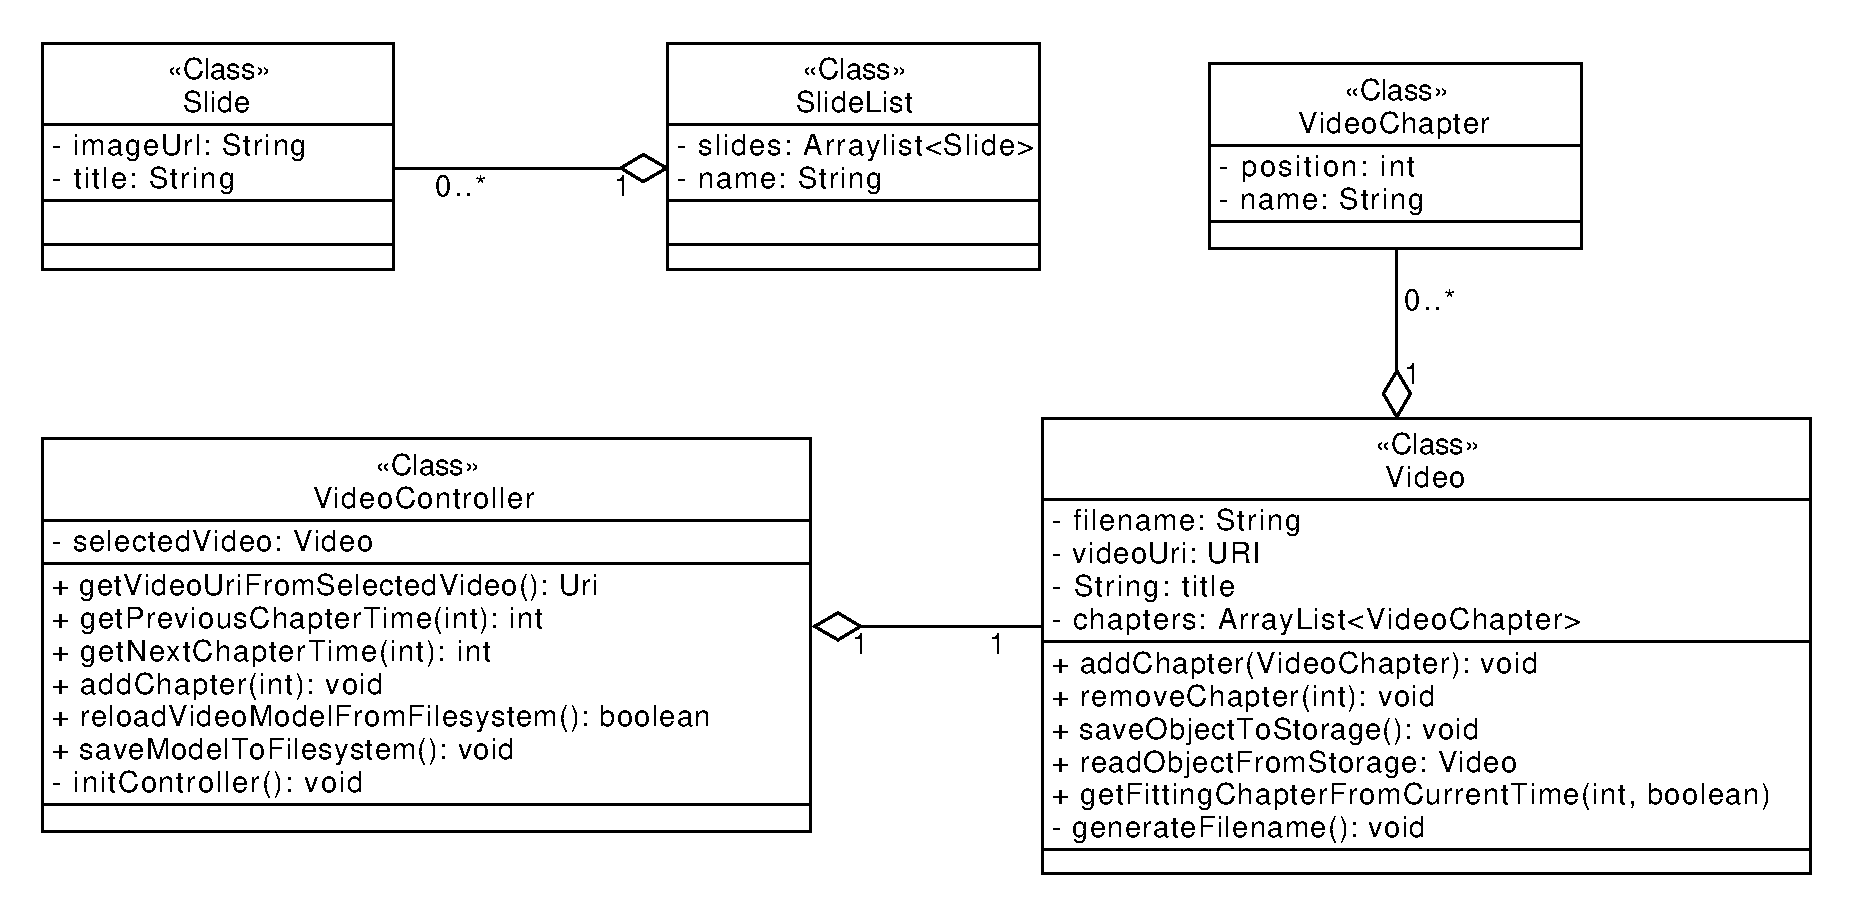
\includegraphics[width=1\textwidth]{data/bilder/Klassendiagramm.pdf}
    \caption{Klassendiagramm der Modelklassen sowie der Controllerklasse}
    \label{fig:Klassendiagramm}
\end{figure}

Die Slides sowie das Video können per Link auf ein JSON-Codiertes Model eingelesen werden. Die Struktur der JSON-Objekte ist in Listing \ref{lst:json_video} und \ref{lst:json_slides} dargestellt.
%
%
%
% - - - - - Programmlogik - - - - - - - - 
%
%
%
\subsection{Programmlogik (Controller)}
Die Programmlogik der Videofunktionalität wird durch einen Controller (vgl. Abbildung \ref{fig:Klassendiagramm}) durchgeführt. Dieser kapselt das Model, also ein Objekt der Klasse Video namens \enquote{selectedVideo}. Mittels verschiedener öffentlicher Methoden kann die Programmlogik realisiert werden. 

\texttt{getVideoURIFromSelectedVideo()} liefert zum gekapselten Model eine Java-URI, die anschließend in der View eingebunden werden kann.

\texttt{getPreviousChapterTime(int)} und \texttt{getNextChapterTime(int)} liefern das nächste Kapitel sowie das vorherige Kapitel abhängig von einer aktuellen Zeit. 

\texttt{addChapter(int)} fügt ein Kapitel zur übergebenen Zeit zum gekapselten Video hinzu. 
\texttt{reloadVideoModelFromFilesystem()} und \texttt{saveModelToFilesystem()} laden bzw. speichern das Model in serialisierter Form im Dateisystem.

Die Slideshow wird per HTTP-Request geladen und aus einem JSON-Objekt (vgl. Listing \ref{lst:json_slides}) in ein Java-Objekt umgewandelt. Es ist ebenso möglich, eine Slideshow aus einem auf einem externen Server liegenden JSON-Datei per QR-Code zu laden. Die Bilder der Slideshow werden von einem Server geladen.

Videos können ebenfalls per HTTP-Request geladen werden und aus einem JSON-Objekt (vgl. Listing \ref{lst:json_video}) in ein Java-Objekt umgewandelt. 

\begin{minipage}{\linewidth}
\begin{lstinputlisting}[%
    caption={JSON-Struktur des Videos},%
    captionpos=b, %
    label={lst:json_video},%
    language=json,%
    firstnumber=1, %
    basicstyle=\scriptsize, %
    breaklines=true]
{sourcecode/jsonStruktur_video.json}
\end{lstinputlisting}
\end{minipage}
%
\begin{minipage}{\linewidth}
\begin{lstinputlisting}[%
    caption={JSON-Struktur der Slides},%
    captionpos=b, %
    label={lst:json_slides},% 
    language=json,%
    firstnumber=1, %
    basicstyle=\scriptsize, %
    breaklines=true]
{sourcecode/jsonStruktur_slides.json}
\end{lstinputlisting}
\end{minipage}
%
%
%
% - - - - - Lokaler Server - - - - - - - - 
%
%
%
\subsection{Lokaler Server}
\label{sec:Lokaler_Server}
Als lokaler Server wird ein NodeJs-Server verwendet. Dieser liefert Zugriff auf alle in einem Ordner \enquote{Public} liegenden Dateien. So lassen sich URLs erstellen und per QR-Code von der Smartglass aus laden, die direkte Links zu Dateien enthalten.

Die Bilder werden zur Anzeige heruntergeladen, die Videos werden gestreamt. Zum Streamen wird die URL des Videos in eine \emph{URI} überführt und dem Android-Videoplayer übergeben. Mithilfe des Videoplayer-Steuerelementes der Android-Api werden die Videoinhalte gestreamt.

Aufgerufen wird der Server über zwei QR-Codes. Der erste Code initialisiert den Server auf dem Client. Die Server-Basis-URL wird zunächst beim Appstart durch einen QR-Code geladen. Dieser enthält die IP-Adresse des Servers sowie den Port, über den die Serveranwendung angesprochen wird. In den QR-Codes von Slidelists sowie Videos werden lediglich die Unterpfade gekapselt, welche zur entsprechenden Datei führen. Innerhalb der Smartglass-Anwendung werden Pfad zum Server und zum Unterpfad zusammengesetzt.

Die Hauptadresse des Servers wird mithilfe einer statischen Hilfsklasse innerhalb des Smartglass-Prototypen gespeichert und ist somit in allen Ansichten der App verfügbar.
%
%
%
%
% - - - - - Evaluation des Prototyps - - - - - - - - 
%
%
%
\chapter{Evaluation des Prototyps}
\label{ch:Evaluation_des_Prototyps}
Zur Evaluation des in Kapitel \ref{ch:Prototyp} beschriebenen Prototyps wurde eine Befragung von potentiellen Nutzern, einem Experten im Bereich der AEMP sowie einer Gruppe technisch versierter Personen durchgeführt. Befragt wurden zwei
Mitarbeitende der AEMP, 
der verantwortliche Leiter der AEMP des Uniklinikums Aachen, 
sowie zwei Softwareentwicklerinnen und Softwareentwickler eines spezialisierten Unternehmens (\emph{IT4Process}), welches Software für Kliniken und insbesondere für die AEMP von Kliniken entwickelt, der Chief Information Officer (CIO) des Unternehmens sowie ein englischsprachiger Mitarbeiter mit geringen Deutschkenntnissen.
%
%
%
%
% - - - - - Befragung im Beruflichen Umfeld - - - - - - - - 
%
%
%
\section{Befragung im beruflichen Umfeld}
\label{sec:Befragung_im_Beruflichen_Umfeld}
Zur Evaluation wurde ein Ablaufplan zum Testen des Prototypen sowie ein anschließender Fragenkatalog entwickelt, der auf die zu befragende Person angepasst war. 

Vor dem Interview wurde die betreffende Person gefragt, welche Erfahrung sie bereits mit Smartphone bzw. Smartglass Apps hat. Zu bewerten waren diese beiden Punkte im Bewertungsbereich von 1 bis 10, wobei 10 die höchste Erfahrungsstufe hat.

Der von den Testpersonen durchzuführende Ablauf war stets der gleiche und war in zwei Teile aufgeteilt. Nach einer Einführung der (nicht völlig selbsterklärenden) Funktionen der Brille wurden der Testperson zwei Aufgaben gestellt. Es sollten Slideshow- und Videofunktionalität getestet werden. 

Zunächst sollte der Menüpunkt \enquote{Bilder} aufgerufen werden. In dieser Unteransicht sollte zunächst ein QR-Code eingelesen werden, um eine extern gelagerte Slideshow zu laden. Anschließend sollte eine Bildergallerie geöffnet werden und in dieser vor- \& zurück navigiert werden.

Das Testen der Videofunktionalität war deutlich umfangreicher. Nachdem aus der Hauptansicht der Menüpunkt \enquote{Video} ausgewählt wurde, sollte ein Video aufgezeichnet werden. Anschließend sollte das Video gestartet, pausiert sowie vor- \& zurückgespult werden. Kapitelmarken sollten hinzugefügt und passend benannt werden. Durch Öffnen der Kapitelansicht sollte eines der Kapitel gelöscht und ein anderes ausgewählt werden. Anschließend sollte ein QR-Code eingelesen und das darin gekapselte Video mit seinen Kapitelmarken geöffnet werden. Hier sollten ebenfalls die zuvor erwähnten Funktionen durchgeführt werden. Anschließend sollte die im Speicher des Gerätes abgelegte Aufnahme erneut nachgeladen werden.

Die Bearbeitungszeit der Nutzer wurde hierbei festgehalten. Anschließend wurden Fragen zur Usability der Brille, zum User-Interface und der Funktionalität des Prototypen sowie zur Einschätzung der Technologie im allgemeinen gestellt.

Die Anwenderinnen und Anwender wurden gefragt, wie sie die Sprachsteuerung, den Tragekomfort sowie die Einsetzbarkeit der Brille in der AEMP einschätzen. Wünsche zur Usability der Brille wurden abgefragt. Zum User Interface des Prototypen wurde abgefragt, ob das Design ansprechend und selbsterklärend ist, die App übersichtlich und die Steuerelemente groß genug sind. Die Funktionalität des Prototypen wurde mit der Frage nach der praktischen Einsetzbarkeit der Funktionalitäten der App (Slides/ Video) sowie nach einer fehlerfreien Funktionalität der App abgefragt. Um eine professionelle Einschätzung der Technologie einzuholen wurde gefragt, ob die Technologie der Smartglasses und des Prototypen im speziellen als Zukunftstechnologie angenommen wird, ob der Einsatz in der AEMP empfehlenswert ist und wo sie in der AEMP eingesetzt werden können. Ebenfalls wurden die Einschätzung der technischen Beschränkungen von Smartglasses in Bezug auf den Einsatz sowohl im Bereich der AEMP, als auch allgemeiner Natur, erfragt. Abschließend wurde die Einsetzbarkeit von Augmented- und Assisted Reality gegenüber gestellt und diskutiert, welche Technologie besser und in welchem Bereich einsetzbar wäre.
%
%\insertMore{Befragung im Beruflichen Umfeld}
%
%
%
% - - - - - Auswertung der Ergebnisse - - - - - - - - 
%
%
%
\subsection{Beschreibung der Interviews}
\label{sec:Beschreinung_der_Interviews}
Im Folgenden werden die durchgeführten Interviews zusammengefasst. Anschließend werden die Interviews ausgewertet und die entscheidenden Erkenntnisse herausgearbeitet.
%
% - - - - - Leiter der AEMP - - - - - - - - 
%
\subsubsection{Leiter der AEMP}
%
Der AEMP-Leiter beschrieb seine Erfahrung mit Smartphones mit dem Punktwert 5, die Erfahrung mit Smartglasses mit 2.

Die Sprachsteuerung der Brille beschrieb er als angenehm, besonders die schnelle Reaktionszeit wurde positiv bewertet. Insgesamt wurde die Brille jedoch als zu schwer wahrgenommen, ein 8 stündiger Einsatz nicht als realistisch eingeschätzt. Dies wurde jedoch lediglich auf dieses Modell (hmt-1) bezogen, andere Smartglasses mit geringerem Gewicht wurden aus Erfahrung des AEMP-Leiters als geeigneter eingeschätzt.

Die Brille könne durchaus im unreinen und reinen Bereich eingesetzt werden. Kritisch betrachtet wurde die Problematik des Einsatzes mit einer Gleitsichtbrille, da diese im Test zu Problemen des scharfen Sehens führte.

Gestensteuerung wurde als nicht sinnvoll eingeschätzt, reine Sprachsteuerung jedoch sehr begrüßt. Besonders die Möglichkeit, freihändig arbeiten zu können, wurde hervorgehoben. Externe Peripheriegeräte wie ein externer Barcodescanner oder ein Monitor wurden als positiv bewertet.

Das Design des Prototypen wurde als überaus gelungen bezeichnet, die App sei einfach und schlicht gehalten sowie einfach zu bedienen. Die Idee das Design, an die bereits bestehende Software der AEMP anzupassen und so eine durchgängige Benutzererfahrung zu gewährleisten, wurde als Anregung einer potentiellen Weiterentwicklung des Prototypen gegeben. Trotz der als intuitiv beschriebenen Benutzeroberfläche wurde angemerkt, dass wohl eine gewisse Einarbeitungszeit vonnöten sei. Angeregt wurde, die Texte nach einer Einarbeitungszeit völlig auszublenden und auf die Erfahrung der Mitarbeiter zu setzen, welche die Bedienung dann beherschten. 

Der Prototyp sei durchaus in seiner Funktionalität einsetzbar. Die Sprachbefehle sollten jedoch einheitlicher gestaltet werden. Eine Kombination von Slideshows und Videos sei denkbar und wünschenswert. Hervorgehoben wurde zudem die nötige Akzeptanz durch die Mitarbeiter und die Bedeutung eines ansprechenden Designs der App, um diese Akzeptanz zu fördern.

Der Prototyp habe fehlerfrei funktioniert. Es sei zu keinen Problemen in der Bedienung gekommen.

Die Frage, ob es sich bei dieser Technologie um eine Zukunftstechnologie handle wurde klar mit ja beantwortet. Der Nutzen der Anwendung sei klar zu erkennen, die Auswahl der Brille jedoch entscheidend. Es solle eine leichte Brille gewählt werden, welche zudem mindestens einen 8 Stunden andauernden Arbeitstag ohne Akkuprobleme überstehen könne. Welche Brille eingesetzt werde, hinge völlig von dem Anwendungszweck ab. So sei ebenfalls der Einsatz \emph{echter} AR-Brillen denkbar, jedoch müsse die entsprechende Brille dann auch die äußeren Anforderungen erfüllen. Eine Sprachsteuerung der Brille und somit das beidhändige Arbeiten wurde als absolut notwendig beschrieben. 

Der Einsatz einer Smartglass mit den im Prototypen dargestellten Funktionen sei sowohl im Reinen als auch im Dekontaminationsbereich sinnvoll. Als weitere Einsatzgebiete wurden der Zentral-OP sowie Schulungen der AEMP herausgestellt. Ärzte seien zum Teil nicht mit modernen Instrumenten und deren Verwendung vertraut. Eine Smartglass könne hier helfen. Die Kommunikation zwischen Außendienstmitarbeitern und einem Arzt könne ebenfalls durch Smartglasses verbessert werden. Angeregt wurde zudem die Remotesteuerung der Brille durch Vorgesetzte.

Grenzen des Einsatzes seien für ihn nicht absehbar, da ihm der nötige Erfahrungsschatz fehle.

Ein Vergleich mit der ihm bekannten Microsoft Hololens ergab, dass durch diese intensive Schulungen und vielfältige Einsatzmöglichkeiten in der AEMP denkbar seien. Der Preis spiele dabei keinerlei Rolle. Problematisch sei bei der Hololens jedoch die mangelnde Sterilisierbarkeit.

Eine Smartglass müsse die strengen Validierungsprozesse der AEMP durchlaufen und neue Standards dafür definiert werden. So könne er sich vorstellen, dass eine reine Wischdesinfektion der Brille bei entsprechender Dokumentation und Definition in den Validierungsstandards des Uniklinikums ausreichen könnte.

Je nach Anwendungszweck müsse also eine andere Smartglass eingesetzt werden. So habe jede Brillenart (Assisted Reality und Augmented Reality) ihre Vorteile. Eine Assisted Reality Smartglass mit ihrem relativ kleinen Bildschirm könne ebenso eingesetzt werden wie eine AR-Brille. Dabei sei eine Assisted Reality Brille durch die Sterilisierbarkeit und das vergleichsweise geringe Gewicht zu bevorzugen, wie auch die geringere Ablenkung durch ein transparentes bzw. kleineres Display.
%
% - - - - - Mitarbeiterin der AEMP - - - - - - - - 
%
\subsubsection{Mitarbeiterin der AEMP}
%
Eine relativ junge Mitarbeiterin (etwa 30 Jahre) beschrieb ihre Erfahrung mit Smartphones als durchschnittlich (etwa 6), Smartglasserfahrung war nicht vorhanden (1).

Die Sprachsteuerung der Brille sei leicht und einfach, der Tragekomfort jedoch sehr unangenehm und drückend. Zudem habe sie Kopfschmerzen und Konzentrationsprobleme gehabt.

Die Einsetzbarkeit innerhalb der AEMP beschrieb sie als kritisch und pessimistisch, da fast alle Funktionen der Brille auch an einem stationären Computer durchgeführt werden könnten. 

Beim Einsatz einer Smartglass sei eine Steuerung per Gesten wünschenswert, Toucheingaben wurden zudem als sinnvoll, ein externer Scanner jedoch als überflüssig angesehen. Externe Monitore könne sie sich sehr gut vorstellen. Die Datenbrille habe ein zu kleines Display und die Ränder der Brille seien, wenn dies auch der \enquote{schweren} Einstellbarkeit geschuldet sein könne, unscharf und dadurch Texte der Ränder schwer lesbar.

Die praktische Einsetzbarkeit der Brille sah sie als kritisch an. So könne sie sich den Einsatz einer Brille, welche ein Display an nur einem Auge habe, nur schwer vorstellen, da dies zu einer Überforderung der Mitarbeiter führte und sehr anstrengend sei. Des Weiteren wies sie auf die mögliche und potentiell gefährliche Strahlung der WLAN- und Bluetoothmodule hin.

Der Prototyp habe fehlerfrei funktioniert. Besonders positiv sei die Videofunktion der Brille, da es so möglich sei, ähnlich einer ihr bekannten Kamera namens \emph{Gopro}, Videos im Blickfeld des Nutzers aufzuzeichnen. 

Ob es sich bei der im Prototypen beschriebenen Technologie jedoch um eine Zukunftstechnologie handle, sei für sie schwer einzuschätzen. Sie stünde dem beschriebenen Prototyp sehr kritisch gegenüber und sehe, dass eher die Nachteile einer solchen Technologie überwögen. Zudem sei die gefährliche Strahlung nicht zu unterschätzen. Die im Prototyp beschriebene Technologie und Funktionalität sei grundsätzlich sinnvoll. Der Einsatz im reinen wie unreinen Bereich der AEMP sei gleichermaßen kritisch zu beurteilen, da eine Ablenkung durch die Smartglass zu schwerwiegenden Fehler führen könne.

Der Einsatz einer Offline-Version der Brille wertete sie positiv, da so die Strahlungsangst überwunden werden könne. Ob der Einsatz einer \emph{echten} AR-Brille sinnvoller sei könne sie nicht beantworten.
%
% - - - - - Mitarbeiter der AEMP - - - - - - - - 
%
\subsubsection{Mitarbeiter der AEMP}
%
Ein etwa 50 Jahre alter Mitarbeiter mit großer Berufserfahrung beschrieb seine Kenntnisse und Erfahrungen mit Smartphones als überdurchschnittlich (etwa 7) sowie die Erfahrung mit Smartglasses als nicht vorhanden (1).

Die Sprachsteuerung der Brille wurde als gewöhnungsbefürftig, jedoch als durchaus erlernbar beschrieben. Die Sprachsteuerung funktioniere nicht immer wie gewünscht auf anhieb, sei jedoch durchaus zufriedenstellend. Auf den Tragekomfort der Brille sei nicht geachtet worden und daher nicht beantwortbar. Den Einsatz der Brille in der AEMP könne er nicht beurteilen, jedoch sei grundsätzlich solch eine Technologie in der Theorie vorstellbar. Positiv sei, dass so ohne Einsatz der Hände ein Computer bedient werden könne. So sei besonders im Reinbereich der AEMP ein beidhändiger Einsatz zwingend nötig, was bei den bisherigen Technologien nicht möglich sei. 

Externe Peripheriegeräte seien durchaus denkbar, da besonders ein externer Monitor die Funktionen der Brille deutlich erweitern könne. Unnötig sei jedoch der Einsatz eines externen Barcode oder QR-Code-Readers.

Das Design des Prototypen wurde als überaus ansprechend jedoch für unerfahrene Nutzer als gewöhnungsbedürftig bezeichnet. Ob das User-Interface selbsterklärend sei könne er nicht beurteilen. Die Brille sei nicht ideal eingestellt gewesen. Dadurch seien die Ränder der Anwendung nicht sichtbar gewesen. Bei korrekter Einstellung der Brille sei das User-Interface jedoch sehr gut bedienbar. Um die Anwendung gut einsetzen zu können sei eine Einarbeitungszeit nötig. 

Der Prototyp sei sicherlich praktisch einsetzbar und biete eine deutliche Erleichterung im Arbeitsalltag der Mitarbeiter. Es sei jedoch eine kurze Anleitung und ausführlichere Erklärung der Anwendung nötig. Nach längerer, alltäglicher Nutzung, ginge die Bedienung jedoch sicherlich \enquote{ins Blut über} und sei dann sicherlich auch einfacher zu bedienen. 

Als negativ wurde der kleine Bildschirm der Brille angemerkt. Ob es sich um eine Zukunftstechnologie handle wurde klar mit ja beantwortet. Der Prototyp habe \enquote{Hand und Fuß}. Kritisch angemerkt wurde jedoch, dass bei einem Ausfall der Netzwerkverbindung die Arbeit in der AEMP nicht mehr möglich sei und so eine starke Abhängigkeit von der Technik entstünde.

Der Einsatz in der AEMP wurde sehr positiv beurteilt und sowohl im reinen wie auch im unreinen Bereich ein Einsatz als möglich gesehen.
%
% - - - - - Softwareentwicklerin IT4Process - - - - - - - - 
%
\subsubsection{Softwareentwicklerin von IT4Process}
%
Eine Mitarbeiterin von IT4Process, einem Unternehmen welches auf Software für Kliniksoftware und insbesondere für die AEMP spezialisiert ist, schätzt ihre Erfahrung mit Smartphones auf sehr erfahren ein (9-10), ihre Erfahrung mit Smartglasses schätzt sie als mittelmäßig (etwa 3-4) ein. 

Die Benutzung der Brille wurde als angenehm und einfach zu steuern empfunden. Die Sprachsteuerung habe fehlerfrei funktioniert. Kritisch angemerkt wurde, dass bei zu ähnlichen Worten möglicherweise das falsche Wort gewählt werde. Der Tragekomfort der Brille wurde als ausreichend beschrieben, was jedoch bei einem 8 Stündigen Einsatz möglicherweise kritischer sein könnte. Der Tragekomfort wurde mit dem einer schweren Basecap verglichen. Bei der Nutzung einer Gleit- oder Lesebrille könne die Brille evtl. zu Problemen führen. Bei gesunden Augen sei dies jedoch kein Problem. Sie schätze es so ein, dass eher junge Mitarbeiter der AEMP die Brille nutzen sollten. Die Nutzung mit einem Auge sei gewöhnungsbedürftig und könne möglicherweise zu Kopfschmerzen führen. Begrüßt wurde hier die Funktionalität der Brille, dass der Bügel der Brille gewechselt werden könne und so zwischen den Augen gewechselt werden kann. Es wurde angemerkt, dass möglicherweise ein transparentes Display Kopfschmerzen und Ermüdungserscheinungen des Auges ebenfalls verringern könnten.

Ermüdung oder Kopfschmerzen wurden nicht festgestellt. Die Sorge vor einer \enquote{gefährlichen Strahlung} bestünde ihrer Meinung nach nicht.

Der Einsatz in der AEMP wurde als potentiell möglich eingeschätzt. Hervorgehoben wurde die Tatsache, dass die Hände bei der Benutzung frei seien. Die Sprachsteuerung sei dabei besonders praktisch und könne möglicherweise durch Kopfgesten ergänzt werden. Eine Sprachsteuerung solle über eine individuelle Sprachsteuerung, die auf die Stimme des Nutzers personalisiert sei, ergänzt werden. Dadurch könnten Fehler vermieden werden.

Einsatz von Peripheriegeräten wie Monitor oder Bar- und QR-Codescanner wurden begrüßt.

Der Prototyp sei selbsterklärend und erinnere an Apps bekannter mobiler  Betriebssysteme wie Android oder iOS. Die Slideshow lasse sich so leicht bedienen wie eine Powerpoint-Präsentation. Positiv hervorgehoben wurde die Übersichtlichkeit der Bedienelemente. So sei die Anordnung intuitiv und die Wahl einer Links-Rechts-Trennung sehr ansprechend. Die Anzeige vieler Steuerelemente sei besser, als viele Untermenüs. Dabei komme es natürlich darauf an, wie geübt ein Nutzer mit Software sei. Die Elemente seien groß genug. 

Der Prototyp wurde als überaus sinnvoll einsetzbar beschrieben. Der Einsatz des Prototypen bringe eine Fehlerreduktion mit sich und vermöge Unsicherheiten im Alltag der Mitarbeiter zu reduzieren. Zudem sei der Einsatz des Prototypen eventuell für schüchterne Mitarbeiter besonders gut geeignet, da so Unsicherheiten ohne Kommunikation mit Kollegen geklärt werden könnten.

Der Prototyp habe fehlerfrei funktioniert und wurde grundsätzlich sehr positiv aufgenommen. Die klare Trennung von Slideshow- und Videofunktionalität wurde begrüßt, wobei angeregt wurde, die Anwendung um die Möglichkeit von Screenshots der Videos zu ergänzen. So könnten Slideshows mit Videos verbunden werden. Ebenso wurde angeregt, die Möglichkeit zum Versenden von Videos zu ergänzen.

Die Frage, ob der Prototyp eine Zukunftstechnologie beschreibe wurde klar mit ja beantwortet. Die Möglichkeiten des Einsatzes seien sehr vielfältig. Im beruflichen Kontext seien auch die im privaten Umfeld hohen Datenschutzrechtlichen Bedenken nicht so relevant, da eine vorherige Einwilligung der betroffenen Personen eingeholt werden könne. Der Aspekt der freien Hände sei besonders hervorzuheben. Der Prototyp sei bereits jetzt besonders ausgereift und für einen Prototpen sehr funktionell ausgestattet.

Die technischen Grenzen wurden eher auf der Seite der Brille als auf Anwenderseite gesehen. So sei die Sprachsteuerung leicht durch externe Befehle manipulierbar und würde leicht irritieren. Hier sei seitens der Brillenhersteller dringend Nachbesserungsbedarf. 

Der Unterschied zwischen \emph{echter} AR-Brillen und Assistent Reality Brillen war bekannt, ebenso die Microsoft Hololens. Die Hololens wurde als kritisch beurteilt, da der Einsatz dieser AR-Brille eine zu große Ablenkung für die Mitarbeiter darstellte und außerdem sei sie zu schwer. Ebenso sei der Effekt der Virtual Sickness nicht zu ignorieren. Der Vorteil von Assistent Reality Brillen sei die leichte Bedienbarkeit für die Nutzer und das geringere Gewicht der Brille.
%
% - - - - - Fremdsprachiger Softwareentwickler IT4Process - - - - - - - - 
%
\subsubsection{Fremdsprachiger Softwareentwickler von IT4Process}
%
Ein englischsprachiger Mitarbeiter von IT4Process, welcher als nicht-Muttersprachler nur geringe Deutschkenntnisse hatte, wurde ebenfalls befragt. Laut seiner Selbsteinschätzung besitzt er fortgeschrittene Kenntnisse im Umgang mit Smartphones (8). Seine Erfahrung mit Smartglasses sind dagegen sehr gering (2). Dieser Nutzer wurde ausgewählt, da viele Mitarbeiter der AEMP nur über geringe Deutschkenntnisse verfügen und daher mit starkem ausländischen Akzent reden.

Im Bereich der Spracherkennung tauchten Probleme auf. Aufgrund der mit starkem Akzent versehenen Aussprache kam es immer wieder zu Verständigungsproblemen. So musste der Proband Sprachbefehle mehrfach wiederholen. Mit einiger Übung wurden diese Probleme jedoch weniger. Zudem musste bei erster Anwendung viele der Funktionen der App erklärt werden, da viele der Befehle nicht sofort verstanden wurden.

Der Tragekomfort sowie das Gewicht wurden als angenehm empfunden. Es bestand jedoch ein Problem mit der vom Probanden getragenen Brille. So konnte aufgrund der eigenen getragenen Brille das Bild der Smartglass nicht scharf fokussiert werden.

Das Design des Prototypen wurde als sauber und selbsterklärend bezeichnet. Angeregt wurde, dass besser Buttons mit Rand benutzt werden sollten, da nicht genau klar sei, was Buttons und was Text ist. Steuerelemente seien groß genug sowie übersichtlich angeordnet. Übermüdung oder Kopfschmerzen traten nicht auf. Der Prototyp wurde als gut benutzbar beschrieben und sei mit etwas Hilfe auch gut verständlich. Er sei nach der Einweisung auch selbstständig nutzbar.

Problematisch war der hmt-1-Befehl \enquote{Hauptmenü}, welcher die App vollständig beendet, sodass der lokale Server neu initialisiert werden müsste.
%
% - - - - - Softwareentwickler von IT4Process - - - - - - - - 
%
\subsubsection{Softwareentwickler von IT4Process}
Ein Softwareentwickler der Firma IT4Process schätzte seine Smartphoneerfahreungen als sehr gut ein (8) sowie seine Smartglasserfahrungen als sehr gering bzw. nicht existent ein (1).

Zunächst stellte er fehst, dass bei nicht optimaler Einstellung der Brille die Ränder nicht sichtbar seien. Die Sprachsteuerung wurde als teilweise schwierig bis nicht funktionierend beschrieben. Sprach er langsam und ordentlich sei die Spracherkennung erfolgreich verlaufen. Die Brille wurde als bequem beschrieben, der 8 Stündige Dauereinsatz jedoch in Frage gestellt. Die Tatsache, dass ein Auge permanent mit einem Display bedeckt sei, wurde stark kritisiert. Ein transparentes Display könne hier Abhilfe schaffen.

Der Einsatz von Smartglasses in der AEMP wurde als grundsätzlich sinnvoll erachtet, die mögliche Störung und Ablenkung der Mitarbeiter jedoch sehr kritisch gesehen. Die 3D-Sicht des Auges sei stark eingeschränkt und behindere so bei filigranen Tätigkeiten, da die Präzision eingeschränkt sei.

Gestensteuerung sowie Kopfbewegungssteuerung wurden als sinnvoll angesehen, wohingegen Touch-Steuerung abgelehnt wurde. Als Peripheriegeräte wurden externe Scanner sowie Monitore für sinnvoll befunden.

Das Design des Prototypen wurde als selbsterklärend beschrieben. Es sei jedoch nicht immer klar, welche Funktionen wie erreichbar seien, was zu einer Überforderung führe. Die Verteilung der Steuerelemente sei nicht immer perfekt und daher etwas verwirrend. Die Elemente seien jedoch gut lesbar.

Als praktisch einsetzbar wurden die Aufnahme und das Abspielen von Videos sowie das Setzen von Kapitelmarken bezeichnet. Statt Slideshows wurden Videos als deutlich sinnvoller angesehen. Die Funktionalität des verlangsamten Abspielens habe gefehlt. Positiv wurde die Strukturierung sowie die Ebenenanzahl beschrieben. Man wisse stehts wozu welche Funktionalität geeignet sei.

Smartglasses wurden als klare Zukunftstechnologie bezeichnet, die verwendete hmt-1 jedoch nicht, da die Spracherkennung nicht genügend und die Displayschärfe nicht ausreichend sei. Der Prototyp beschreibe ebenfalls eine Zukunftstechnologie. Die Funktionen des Prototypen wurden für den Einsatz bei Anleitungen, beim Anlernen neuer Mitarbeiter sowie für Schritt für Schrittanleitungen gesehen. Die Anwendung könne sowohl im Reinen als auch im Unreinen Bereich Verwendung finden. Andere Anwendungsbereiche seien Gebäudeführung sowie alle Arbeiten, bei denen Angestellte nachträglich geschult werden müssten. 

Der Technologie seien aber mannigfaltige Grenzen gesetzt: So sei die Bandbreite des WLAN, die Positionsbestimmung ohne GPS (in Gebäuden), die Größe der Instrumente sowie der Akku limitierende Faktoren. Der Akku müsse zudem mindestens 8 Stunden halten, was nach mehrjähriger Nutzung problematisch werde. So müsse eine Aufladeinfrastruktur geschaffen werden.

Der Vergleich von AR und Assisted Reality zeige, dass es stark auf den Anwendungsfall ankomme. So benötigten AR-Brillen deutlich mehr Strom (gesteigerter Akkuverbrauch) sowie mehr Rechenleistung. Asssted Reality Brillen hätten den Vorteil geringerer Rechenleistung bei verringerter Ablenkung des Nutzers zu haben.
%
% - - - - - Chief Information Officer IT4Process - - - - - - - - 
%
\subsubsection{Entwicklungsleiter IT4Process}
Der Entwicklungsleiter der Firma IT4Process beschreibt sich selbst als sehr erfahren mit Smartphones (8) und mittel erfahren mit Smartglasses (4).

Die Sprachsteuerung der hmt-1 wurde als \enquote{erstaunlich gut} bezeichnet. Sie übertraf die Erwartungen des Probanden. Der Tragekomfort der Brille wurde positiv aufgenommen. So wurde die Brille als gut ausbalanciert bezeichnet. Das Display wurde kritisch betrachtet. So wäre eine Abwägung zwischen einen halbtransparenten und transparenten Display zu treffen. 

Der Einsatz in der AEMP wurde differenziert betrachtet: die Tatsache, dass Nutzer sich ins Gesicht fassen müssten, um die Brille zu justieren, wurde kritisiert und dass im Reinbereich die Brille nicht wirklich gut einsetzbar sei. Spracheingabe wurde als ermüdend und störend eingestuft, was eine Toucheingabe (möglicherweise mittels Peripheriegeräten) sinnvoll mache. Spracherkennung könne sich gegenseitig behindern, da mehrere Menschen parallel arbeiteten. So könne beispielsweise ein Fußschalter helfen oder andere Peripheriegeräte zur Eingabe (bspw. Touchbar). Externe Scanner wurden genau wie externe Monitore als sinnvoll angesehen. Eine Waage könne ebenfalls eine sinnvolle Erweiterung darstellen.

Das Design des Prototypen wurde mit iOS-Apps verglichen, da es von typischen Android Apps abweiche. Die Farbgebung wurde daher für Androidnutzer als irritierend wahrgenommen, da die Farbgebung anders als typische Android-Apps ausfalle. Zur genaueren Identifikation der Kapitelmarken wurden Screenshots empfohlen, welche neben der Auswahl in der Kapitelauswahl angebracht werden sollten. Zur Steuerung der App wurde eine Kopfgestensteuerung angeregt, die ein vor- und zurückspulen ermöglichen könne. Auch hier kam es zur falschen Benutzung des hmt-1-Befehls \enquote{Hauptmenü}, was zu einem Beenden der App führte. Die Steuerelemente wurden als groß genug bezeichnet.

Die praktische Einsetzbarkeit wurde vor allem bei Schulungen gesehen. Die App wurde als fehlerfrei bedienbar beschrieben. Als gut wurde die geringe Menütiefe hervorgehoben.

Ob es sich um eine Zukunftstechnologie handle könne der Proband nicht sagen. Es sei noch ein \enquote{weiter Weg} bis zur Marktreife. Der Haupteinsatzort sehe er im Lager und in der Chargenfreigabe der AEMP. Für genauere Anleitungsvideos seien Monitore besser geeignet. Smartglasses und multimediale Anwendungen seien immer da gut einsetzbar, wo kein fester Arbeitsplatz vorhanden sei. So könne freihändig gearbeitet werden.

Grenzen der Smartglass in der AEMP seien durch die beschränkten Möglichkeiten der Interaktion ohne Maus und Tastatur sowie die geringe Auflösung der Kamera gegeben. Die Informationsdichte auf einem kleinen Display sei stark limitiert und bechränke damit die Menge an Informationen, die auf der kleinen Fläche dargestellt werden könne. Positiv sei, dass in der AEMP Aachen beispielsweise nur sehr kleine Bildschirme mit geringer Auflösung eingesetzt würden, was eine Übertragung auf eine Smartglass vereinfache.

Vergleiche zwischen Assisted Reality Brillen und Augmented Reality Brillen zeige, dass die Voraussetzungen (Abwischbar, großes Sichtfeld und leichtes Gewicht) momentan echte AR-Brillen als nicht geeignet klassifizieren, um in der AEMP eingesetzt zu werden. Der Vorteil von Assisted Realitybrillen sei das geringe Gewicht, die Abwischbarkeit sowie die Robustheit der Brille.
%
%
% - - - - - Auswertung der Ergebnisse - - - - - - - - 
%
\subsection{Auswertung der Ergebnisse}
\label{sec:Auswertung_der_Ergebnisse}
%
%
%
Die Erfahrung der Testpersonen mit der verwandten Technologie der Smartphones (oftmals mit dem bekannten Betriebssystem Android) kann als durchaus überdurchschnittlich angesehen werden. So geben alle Testpersonen der AEMP an, über leicht über dem Durchschnitt ($>5$) liegende Erfahrung mit dieser Technologie zu verfügen. Die Erfahrung mit Smartglasses ist jedoch bei fast allen Nutzern nicht vorhanden. Lediglich der Leider der AEMP gab an, geringe (2) Erfahrung mit Smartglasses zu haben. Die befragten Softwareentwickler verfügten berufsbedingt über einen größeren Erfahrungsschatz.

Die Hardware, also die hmt-1 Brille, wurde durchaus kritisch gesehen. So sei sie zu schwer, verursache Kopfschmerzen und wurde zum Teil als unbequem bezeichnet. Das Display wurde als zu klein, schwer einstellbar und nicht scharf beschrieben. Die Einsetzbarkeit der verwendeten Brille wurde ebenfalls insgesamt als kritisch angesehen. Der Leiter der AEMP jedoch beschrieb die ihm bekannten anderen Smartglasses (sofern diese sterilisierbar wären) als durchaus geeigneter. So komme es auf das Gewicht der Brillen an. 

Peripheriegeräte seien zum Teil sinnvoll. Monitore wurden insgesamt als gute Erweiterung eingeschätzt. Touch und Gestensteuerung fanden dagegen ambivalente Bewertung der Tester.

Der Prototyp wurde durchgehend positiv angesehen. Besonders der verantwortliche Leiter der AEMP sah eine große Chance der im Prototypen beschriebenen Technologien. So könnten große Arbeitserleichterungen durch den multimedialen Einsatz in der AEMP entstehen. 

Das User Interface des Prototypen wurde ebenfalls durchgehend als ansprechend und größtenteils als selbsterklärend beschrieben. Die Funktionalitäten des Prototypen wurden selbst von der der Technik kritisch gegenüberstehenden Mitarbeiterin der AEMP als sinnvoll angesehen. Das User Interface des Prototypen wurde durchgehend als übersichtlich und ansprechend beschrieben.

Die Funktionalität der Brille sei gut bedienbar und fehlerfrei.

Die Technologie wurde größtenteils als Zukunftstechnologie bezeichnet. Der Einsatz in der AEMP wurde teils zwar als kritisch beurteilt, jedoch grundsätzlich als möglich eingestuft. Der Einsatz im Reinbereich und Dekontaminationsbereich der AEMP sei möglich. Besonders hervorzuheben ist hier die professionelle Einschätzung des Leiters der AEMP und des erfahrenen Mitarbeiters, welche den Einsatz in beiden Bereichen als überaus sinnvoll angesehen haben.

Andere Einsatzmöglichkeiten innerhalb der AEMP wurden als durchaus realistisch eingeschätzt. So wurde vor allem der Aspekt der Schulung und Fortbildung genannt. Hier könnten auch \emph{echte} AR-Brillen eingesetzt werden, welche ansonsten für den ganztägigen Einsatz zu schwer seien.

Die Grenzen der Assisted Reality-Brillen wurden durchaus gesehen. So sei die geringe Displaygröße ein starker limitierender Faktor der Einsatzmöglichkeiten. So kann sich der Leiter der AEMP den Einsatz von \emph{echten} AR-Brillen besser vorstellen, sofern die äußeren limitierenden Faktoren wie Sterilisierbarkiet eingehalten werden können.

Ob eine \emph{echte} AR-Brille oder eine Assisted Reality Brille mit der im Prototypen dargelegten multimedialen Technologie eingesetzt werde, hänge ganz vom Anwendungszweck ab und sei pauschal nicht zu sagen. Die Vorteile von Assisted Reality-Brillen im Bereich der Medizinprodukteaufbereitung wurden jedoch bei allen Testern positiv beurteilt.

Die Nutzererfahrung war sehr davon abhängig von der Erfahrung der Nutzer mit Smartphones und anderen Smartglasses im Allgemeinen war. So waren erfahrene Nutzer deutlich zufriedener mit der Brille und mit dem Prototypen und konnten wesentlich besser die Relevanz der Software einschätzen. 
%
%
%
%
% - - - - - Fazit - - - - - - - - 
%
%
%
\chapter{Fazit}
\label{ch:Fazit}
\insertMore{Fazit}
% 3 Seiten
%
\chapter{Ausblick}
%
% - - - Literaturverzeichnis - - - 
\printbibliography[title={Literaturverzeichnis}]
%
% - - - Abbildungsverzeichnis - - - 
\listoffigures
%
% - - - Codeverzeichnis - - - 
\lstlistoflistings
%
%
\end{document}